

\chapter{Potencial de Yukawa}


\section{Ecuaci\'on de Klein-Gordon}
\label{sec:ecuacion-de-klein}
%to_en: From the scalar component we obtain from eq.~\eqref{eq:27}, with the Lagrangian for the Klein-Gordon equation for a real scalar field $\phi=A^0$
La interacci\'on entre un prot\'on y un neutr\'on fue determinada experimentalmente por Tomonaga en 1934 \cite{history}
\begin{align}
\label{eq:243}
  V(r)={A}\frac{e^{-r/\Lambda }}{r}\,,
\end{align}
con
\begin{align}
  \label{eq:245}
  \Lambda\approx1/(7\times10^{12}\,\text{cm}^{-1})=1.43\times10^{-13}\,\text{cm}=1.43\times10^{-15}\,\text{m}\,.
\end{align}
Consideremos el principio de incertidumbre
\begin{align}
  \Delta x\, \Delta p &\geq \frac{\hbar}{2}\nonumber\\
\Delta t\, \Delta E&\geq\frac{\hbar}{2}\,.
\end{align}
La segunda relaci\'on de incertidumbre
aplicada a la ecuación de Klein-Gordon~\cite{Aitchison:2003tq}, brinda un nuevo entendimiento de la relaci\'on entre el rango y la masa en ec.~\eqref{eq:243}. $\Delta t$ es el tiempo que el sistema cu\'antico interact\'ua con el aparato de medida y $\Delta E=\hbar/(2\Delta t)$ es el error m\'\i nimo que se obtiene en la medida de la energ\'\i a, tal que $E=E_0\pm\Delta E$. Es decir, para medir la energ\'\i a con una precisi\'on $\Delta E$, uno necesita un tiempo mayor que $\hbar/(2\Delta E)$.

Si $\Delta E< mc^2$ eso quiere decir que podemos medir la cantidad $mc^2$ con alguna certeza. Es decir que una part\'\i cula de masa $m$ se puede llegar a observar. Si $\Delta E>mc^2$ entonces una part\'\i cula de masa $m$ puede existir durante un tiempo $\Delta t$. A tal part\'\i cula se le llama virtual porque no es observable. 

El momentum de una part\'\i cula de n\'umero de onda $k$ es $p=\hbar k$, de modo que la incertidumbre en el momentum para una part\'\i cula relativista es
\begin{align}
  \Delta p=\hbar\, \Delta k \approx\hbar\, \frac{\Delta\omega}{c}=\frac{\Delta E}{c}
\end{align}

Si la masa de la part\'\i cula es cero entonces $E$ puede tender a cero, que corresponde al caso de un part\'\i cula no masiva con un momentum tendiendo a cero. La cantidad por la cual la conservaci\'on de energ\'\i a es violada, $\Delta E$, tambi\'en puede llegar a ser muy peque\~na. De modo que un fot\'on virtual de frecuencia muy baja puede existir durante un tiempo casi infinito. Durante ese tiempo un fot\'on viajando a la velocidad de la luz podr\'\i a viajar una distancia casi infinita y puede dar cuenta de una interacci\'on de rango infinito. 

Sin embargo, para una part\'\i cula de masa $m$. La violaci\'on de energ\'\i a para producir esta debe ser de al menos $mc^2$, o $\Delta E>mc^2$. Por el principio de incertidumbre la m\'axima distancia que puede recorrer es $\Lambda=c\Delta t$

\begin{align}
\label{eq:244}
  \Lambda \geq & \frac{\hbar c}{2\Delta E}\nonumber\\
  \geq &\frac{c\hbar}{2mc^2}\nonumber\\
  \geq &\frac{\hbar}{2mc}\nonumber\\
  \geq &\frac{1}{2m}\qquad\text{Natural Units} \,.
\end{align}

De la componente escalar de la ecuaci\'on de Proca, \eqref{eq:27}, obtenemos la ecuaci\'on de Klein--Gordon para un campo escalar real $\phi=A^0$,
\begin{align}
  \label{eq:29}
  \mathcal{L}=&\frac{1}{2}\partial^\mu\phi\partial_\mu\phi-\frac{1}{2}m^2\phi^2+\rho\phi
\end{align}
Donde $\rho$ es la densidad de carga que actua como fuente del campo $\phi$.

%to_en: Later we will discuss in detail why $m$ corresponds to the mass of the particle. The idea is that $\phi$ has excitations around the minimum of the potential $V=(1/2)m^2\phi^2$ that have some harmonic oscillator energy, and this energy is equivalent to mass. Note that $m^2\lt 0$ cannot be interpreted as mass. In this case $\phi$ will describe excitations around the flat part of the potential. Since this excitations do not cost energy, they correspond to a non-massive particle.
Posteriormente discutiremos en detalles porque $m$ corresponde a la masa de la part\'\i cula. La idea b\'asica es que $\phi$ tiene excitaciones alrededor del m\'\i nimo del potencial $V=(1/2)m^2\phi^2$ que corresponde a la energ\'\i a de un oscilador arm\'onico. Esta energ\'\i a es equivalente a masa. Note que $m^2\lt 0$ no puede interpretarse como masa. En este caso $\phi$ describir\'a excitaciones alrededor de la parte plana del potencial. Como estas excitaciones no cuestan energ\'\i a, corresponde a una part\'\i cula sin masa. 

%to_en: The field $\phi$ can be thought of as arising from a source in much the same way as the electromagnetic fields arise from charged particles; as for the electromagnetism, en esta secci\'on we can consider the fields without concerning ourselves with the sources. 
El campo $\phi$ puede pensarse como proveniente de una fuente de la misma manera como el campo electromagn\'etico surge de part\'\i culas cargadas. Como en el caso del electromagnetismo, en esta secci\'on podemos considerar los campos sin preocuparnos de las fuentes. 
En tal caso tendremos una teor\'\i a en la cual el campo escalar juega el papel de part\'\i cula mediadora de la interacci\'on.

Si el campo escalar se generaliza para que pueda tener otros n\'umeros
cu\'anticos, como carga el\'ectrica, entonces estos pueden ser las fuentes
de las respectivas cargas y corrientes en la ecuaciones para campos
vectoriales. Esto se estudiar\'a en la
secci\'on~\ref{sec:camp-escal-compl}. En tal caso podr\'\i amos tener por
ejemplo ``\'atomos'' formados de part\'\i culas escalares que se excitan
emitiendo fotones.


En las secciones~\ref{sec:ecuac-covar} y \ref{sec:ecuacion-de-proca},
hemos visto que el Lagrangiano en ec.~\eqref{eq:29} da lugar a las
ecuaciones de Klein-Gordon en presencia de una densidad de carga
\begin{equation}
  \label{eq:30}
  (\Box+m^2)\phi=\rho
\end{equation}
De acuerdo a la ec.~\eqref{eq:28}, tenemos
\begin{align}
\mathcal{L}_{\text{free}}&=\frac{1}{2}\partial_\mu\phi\partial_\mu\phi-\frac{1}{2} m^2\phi^2\nonumber\\
\label{eq:31}
\mathcal{L}_{\text{int}}&=\rho\phi
\end{align}
En analog\'\i a con el electromagn\'etismo donde las densidades de carga y
corrientes son la fuente del campo $A^\mu$, podemos pensar en $\rho$ como
la fuente del campo $\phi$. En el caso del electromagnetismo el an\'alisis
de las ecuaciones de Maxwell en forma covariante,
ec.~\eqref{eq:nohomME2}, para las componentes $A^0$ y $J^0$, en el
gauge de Coulomb:
\begin{equation}
  \label{eq:32}
  \boldsymbol{\nabla}\cdot\mathbf{A}=0,
\end{equation}
da lugar a la Ley de Coulomb, que corresponde a una interacci\'on de
rango infinito \cite{Gross}. Veremos a continuaci\'on que un an\'alisis
similar para un campo escalar masivo (o para la componente cero de un
campo vectorial masivo) da lugar a una interacci\'on de corto rango.

Consideremos el caso m\'as simple de una fuente puntual para el campo
$\phi$:
\begin{equation}
  \label{eq:33}
  \rho(x)=g\delta(\mathbf{x})
\end{equation}
donde $g$ es una constante. Entonces $\rho$ es independiente del tiempo y
genera un campo (un potencial) independiente del tiempo. Entonces,
como:
\begin{equation*}
  \frac{\partial\phi}{\partial t}=0,
\end{equation*}
tenemos
\begin{equation}
  \label{eq:34}
  (-\nabla^2+m^2)\phi(\mathbf{x})=g\delta(\mathbf{x})
\end{equation}
Para resolver la ecuaci\'on diferencial es m\'as conveniente transformar
$\phi(\mathbf{x})$ al espacio de momentos. Su transformada de Fourier es
\begin{equation}
  \label{eq:35}
  \phi(\mathbf{x})=\frac{1}{(2\pi)^{3/2}}\int d^3k\,e^{i\mathbf{k}\cdot\mathbf{x}}\tilde\phi(\mathbf{k}).
\end{equation}
La transformada inversa es
\begin{equation}
  \label{eq:36}
  \tilde\phi(\mathbf{k})=\frac{1}{(2\pi)^{3/2}}\int d^3x\,e^{-i\mathbf{k}\cdot\mathbf{x}}\phi(\mathbf{x}).
\end{equation}
Ademas tenemos la propiedad
\begin{equation}
  \delta(\mathbf{x})=\frac{1}{(2\pi)^3}\int d^3k\,e^{i\mathbf{k}\cdot\mathbf{x}}.
\end{equation}
Reemplazando ec.~\eqref{eq:35} en \eqref{eq:34}, tenemos
\begin{align}
\frac{1}{(2\pi)^{3/2}}\int d^3k(\mathbf{k}^2+m^2)e^{i\mathbf{k}\cdot\mathbf{x}}\tilde\phi(\mathbf{k})&=g\delta(\mathbf{x})\nonumber\\
&=\frac{g}{(2\pi)^3}\int d^3k\,e^{i\mathbf{k}\cdot\mathbf{x}}\nonumber\\
(\mathbf{k}^2+m^2)\tilde\phi(\mathbf{k})&=\frac{g}{(2\pi)^{3/2}}.\nonumber
\end{align}
Entonces
\begin{equation}
  \tilde\phi(\mathbf{k})=\frac{g}{(2\pi)^{3/2}}\frac{1}{\mathbf{k}^2+m^2}.
\end{equation}
Reemplazando en la ec.~\eqref{eq:35} y definiendo $r\equiv|\mathbf{x}|$
\begin{align}
  \phi(\mathbf{x})=&\frac{1}{(2\pi)^{3/2}}\int d^3k\,e^{i\mathbf{k}\cdot\mathbf{x}}
  \left[
    \frac{g}{(2\pi)^{3/2}}\frac{1}{\mathbf{k}^2+m^2}
  \right]\nonumber\\
=&\frac{g}{(2\pi)^{3}}\int d^3k
    \frac{e^{i\mathbf{k}\cdot\mathbf{x}}}{\mathbf{k}^2+m^2}\nonumber\\
=&\frac{g}{(2\pi)^{3}}2\pi\int_0^\infty d|\mathbf{k}|
    \frac{\mathbf{k}^2}{\mathbf{k}^2+m^2}\int_0^\pi e^{i|\mathbf{k}|r\cos\theta}\sen\theta\,d\theta\nonumber
\end{align}
Haciendo el cambio de variables $u=\cos\theta$, $du=-\sin\theta\,d\theta$,
\begin{align}
  \phi(\mathbf{x})=&-\frac{g}{(2\pi)^2}\int_0^\infty d|\mathbf{k}|
    \frac{\mathbf{k}^2}{\mathbf{k}^2+m^2}\int_{1}^{-1}e^{i|\mathbf{k}|ru}du,\nonumber\\
  \phi(\mathbf{x})=&\frac{g}{(2\pi)^2}\int_0^\infty d|\mathbf{k}|
    \frac{\mathbf{k}^2}{\mathbf{k}^2+m^2}\int_{-1}^1e^{i|\mathbf{k}|ru}du.
\end{align}
%\textbf{check minus sign!} 
Ya que  
\begin{equation*}
  \int_{-1}^1e^{i|\mathbf{k}|ru}du=\frac{e^{i|\mathbf{k}|r}-e^{-i|\mathbf{k}|r}}{i|\mathbf{k}|r}
\end{equation*}
\begin{align}
  \phi(\mathbf{x})=&\frac{g}{i(2\pi)^2r}\int_0^\infty d|\mathbf{k}|\,|\mathbf{k}|
    \frac{e^{i|\mathbf{k}|r}-e^{-i|\mathbf{k}|r}}{\mathbf{k}^2+m^2}\nonumber\\
    =&\frac{g}{i(2\pi)^2r}\left(\int_0^\infty d|\mathbf{k}|\,|\mathbf{k}|
\frac{e^{i|\mathbf{k}|r}}{\mathbf{k}^2+m^2}-\int_0^\infty d|\mathbf{k}|\,|\mathbf{k}|
\frac{e^{-i|\mathbf{k}|r}}{\mathbf{k}^2+m^2}\right)\nonumber\\
=&\frac{g}{i(2\pi)^2r}\left(\int_0^\infty d|\mathbf{k}|\,|\mathbf{k}|
\frac{e^{i|\mathbf{k}|r}}{\mathbf{k}^2+m^2}-\underbrace{\int_0^{-\infty}d|\mathbf{k}|\,|\mathbf{k}|
\frac{e^{i|\mathbf{k}|r}}{\mathbf{k}^2+m^2}}_{|\mathbf{k}|\to-|\mathbf{k}|}\right)\nonumber\\
=&\frac{g}{i(2\pi)^2r}\int_{-\infty}^\infty d|\mathbf{k}|\,|\mathbf{k}|
\frac{e^{i|\mathbf{k}|r}}{\mathbf{k}^2+m^2}\nonumber\\
\label{eq:37}
    =&\frac{g}{i(2\pi)^2r}\int_{-\infty}^\infty d|\mathbf{k}|
    \frac{|\mathbf{k}|e^{i|\mathbf{k}|r}}{(|\mathbf{k}|+im)(|\mathbf{k}|-im)}
\end{align}
Definiendo
\begin{equation*}
  f(z)=\frac{ze^{izr}}{z+im}
\end{equation*}
y usando la integral de Cauchy para el contorno correspondiente al semiplano positivo que incluye el polo en $z=im$
\begin{equation}
  \int_C\frac{f(z)}{z-im}dz=2\pi if(im)=2\pi i\frac{im\,e^{-mr}}{2im}=\pi i\,e^{-mr}
\end{equation}
tenemos que
\begin{equation}
 \label{eq:38}
  \phi(\mathbf{x})=\frac{g}{4\pi}\frac{e^{-mr}}{r}
\end{equation}

A la luz de la interacci\'on fuerte, un prot\'on y un neutr\'on son
indistinguibles y son llamados nucleones. En primera aproximaci\'on la
interacci\'on fuerte puede ser tratada como una interacci\'on de Yukawa en
el rango de los fermis entre los nucleones, mediada por mesones, como el pi\'on. Ver sec. 2.2 de \cite{Aitchison:2003tq}.


Para ver esto considere un nucle\'on como fuente de un mes\'on
intermediario. De acuerdo a la ec.~(\ref{eq:38}),
\begin{align}
  \phi(\mathbf{x})&=\frac{g}{4\pi}\frac{e^{-m|\mathbf{x}|}}{|\mathbf{x}|}\nonumber\\
  &=\frac{1}{4\pi}\int d^3x'g\,\delta(\mathbf{x}')\frac{e^{-m|\mathbf{x}-\mathbf{x}'|}}{|\mathbf{x}-\mathbf{x}'|}\nonumber\\
  &=\frac{1}{4\pi}\int d^3x'\rho(\mathbf{x}')\frac{e^{-m|\mathbf{x}-\mathbf{x}'|}}{|\mathbf{x}-\mathbf{x}'|}
\end{align}

\begin{equation}
  \mathcal{L}_{\text{int}}=\phi(\mathbf{x})\rho(\mathbf{x})=\frac{1}{4\pi}\int d^3x'\rho(\mathbf{x})\rho(\mathbf{x}')\frac{e^{-m|\mathbf{x}-\mathbf{x}'|}}{|\mathbf{x}-\mathbf{x}'|}
\end{equation}
\begin{align}
  \mathcal{H}_{\text{int}}&=\frac{\partial\mathcal{L}_{\text{int}}}{\partial(\partial\phi/\partial t)}\frac{\partial\phi}{\partial t}-\mathcal{L}_{\text{int}}\nonumber\\
  &=-\mathcal{L}_{\text{int}}\nonumber\\
  &=-\frac{1}{4\pi}\int d^3x'\rho(\mathbf{x})\rho(\mathbf{x}')\frac{e^{-m|\mathbf{x}-\mathbf{x}'|}}{|\mathbf{x}-\mathbf{x}'|}
\end{align}
\begin{equation}
  \label{eq:39}
  H_{\text{int}}=-\frac{1}{4\pi}\int d^3x\,d^3x'\rho(\mathbf{x})\rho(\mathbf{x}')\frac{e^{-m|\mathbf{x}-\mathbf{x}'|}}{|\mathbf{x}-\mathbf{x}'|}
\end{equation}
El Hamiltoniano de interacci\'on en ec.~(\ref{eq:39}) representa la
interacci\'on entre dos nucleones mediante el intercambio de un mes\'on.
En forma an\'aloga a como dos electrones intercambian un fot\'on mediante
la interacci\'on electromagn\'etica. En el caso de $m=0$,
$H_{\text{int}}$, corresponde a la de energ\'\i a potencial de Coulomb. El
potencial por unidad de carga al cuadrado, puede escribirse como
\begin{equation}
  \label{eq:40}
    V(r)=-\frac{1}{4\pi}\frac{e^{-mr}}{r}
\end{equation}
El potencial en (\ref{eq:40}) recibe el nombre de \emph{potencial de
  Yukawa} y corresponde a una interacci\'on de rango $r\sim1/m$. 

Comparando con la ec.~(\ref{eq:243}) tenemos
\begin{align}
  m\approx&\frac{1}{\Lambda}
\end{align}
que es compatible con la ec.~\eqref{eq:244}. Usando el valor medido de $\Lambda$ en la ec.~\eqref{eq:245}
\begin{align}
  m\approx&\frac{1}{1.43\times10^{-15}m}\frac{1.973\times10^{-16}\,\text{m}}{\text{GeV}^{-1}}\nonumber\\
  \approx&138\,\text{MeV}
\end{align}
La masa del pion $\pi^0$, es $m_{\pi^0}=134.8766(6)\,$MeV.



En el caso general tenemos que $\phi(x)$ satisface la ecuaci\'on de Klein-Gordon en el espacio libre, ec.~\eqref{eq:30}
\begin{equation}
    (\frac{\partial^2}{\partial t^2}-\nabla^2+m^2)\phi=0
\end{equation}
con soluci\'on, 
\begin{equation}
  \phi\propto\exp(i\mathbf{k}\cdot\mathbf{x}-i\omega t)
\end{equation}
que, consistente con la discusi\'on en la secci\'on~\ref{sec:srn}, ec.\eqref{eq:k-gpmu}, da lugar a la condici\'on 
\begin{equation}
  m^2=\omega^2-\mathbf{k}^2.
\end{equation}
De este modo $m$, puede interpretarse como la masa de la part\'\i cula $\phi$.

Para complementar la discusi\'on, condere el caso de un aparato de medida con el m\'\i nimo requerimiento para descubrir el $\pi^0$.
El tiempo que el $\pi^0$ tarda en crurzar del prot\'on al nucle\'on debe ser al menos de $r/c$. El aparato de medida debe operar a una escala de tiempos
\begin{align}
  \Delta t<\frac{r}{c}\,.
\end{align}
La incertidumbre en la enrg\'\i a ser\'a
\begin{align}
  \Delta E\geq \frac{\hbar}{2\Delta t}=\frac{\hbar c}{2r}\,.
\end{align}
Reemplazando $\Delta E=\frac{1}{2}m c^2$ para que la medida $E\pm\Delta E$ sea significativa a dos $\sigma$, tenemos que
\begin{align}
  r\geq \frac{\hbar}{ m c}\,.
\end{align}
De este modo $r$ es la medidad de la separaci\'on entre $n$ y $p$, tal que en el tiempo disponible, el $\pi^0$ pueda robar la energ\'\i a necesaria para llegar a existir y cruzar de uno a otro. Usando $m=138\,$MeV, tenemos 
\begin{align}
  r\geq\frac{1}{0.138}\,\text{GeV}^{-1}\times\frac{1.973\times10^{-16}\,\text{m}}{\text{GeV}^{-1}}=1.43\times10^{-15}\,\text{m}.
\end{align}
El valor obtenido de $\Lambda$ es compatible con $r$. $\Lambda$ es el rango efectivo de la fuerza asociada. 
A continuaci\'on Yukawa considero la posibilidad de que el quantum $\phi$ pudiera ser emitido en la transici\'on $n\to p$, a trav\'es del proceso
\begin{equation}
  \label{eq:154}
  n\to p+\phi^-
\end{equation}
donde la conservaci\'on de la carga determina la carga de $\phi^-$. Sin embargo el proceso viola la conservaci\'on de la energ\'\i a ya que $m_n=939.565\;56(81)\,$MeV, $m_p=938.272\;013(23)\,$MeV, de modo que $m_n\lt m_p+m_\phi$, si $m_\phi\sim100\,$MeV, as\'\i{} esto no puede ocurrir como un proceso real de emissi\'on. Sin embargo, Yukawa not\'o que si \eqref{eq:154} se combina con el proceso inverso
\begin{equation}
  p+\phi^-\to n
\end{equation}
entonces una interacci\'on $n$--$p$ podr\'\i a tomar lugar a trav\'es del mecanismo mostrado en la figura \ref{fig:n-p}(a). Es decir a trav\'es del intercambio de un quantum $\phi^-$. El otro diagrama compatible con la conservaci\'on de la carga tambi\'en aparece en la figura
%noinstiki
\begin{figure} %noinstiki

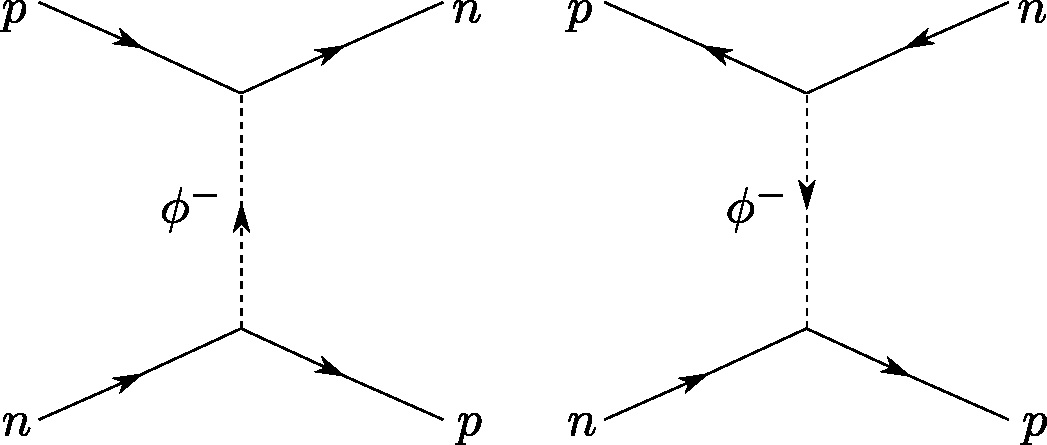
\includegraphics{yukawa-schange} %noinstiki
  \caption{Intercambio de Yukawa de un s\'olo $\phi$} %noinstiki
\label{fig:n-p} %noinstiki
\end{figure} %noinstiki<div id="fig:n-p">Figura: Intercambio de Yukawa</div>
%noinstiki![yukawa-schange](http://gfif.udea.edu.co/figfs/yukawa-schange.png)
%noinstiki


En el espacio de momentos, la cantidad relevante que representa el
intercambio de piones, es la que aparece en la ec.~(\ref{eq:37}) y se
conoce como el \emph{propagador}:
\begin{equation}
\text{propagador:}\qquad \frac{1}{\mathbf{k}^2-m^2}
\end{equation}
En el caso electromagn\'etico tendremos simplemente
\begin{equation}
  1/\mathbf{k}^2.
\end{equation}
Para part\'\i culas $\alpha$ incidiendo sobre un metal y siendo dispersadas por un \'angulo $\theta$ entre $\mathbf{q}$ y $\mathbf{q}'$, tal que se satisface la condici\'on de dispersi\'on el\'astica $\mathbf{q}^2={\mathbf{q}'}^2$ (dispersi\'on de Rutherford)
\begin{align}
  \mathbf{k}^2=(\mathbf{q}-\mathbf{q}')^2=2\mathbf{q}^2(1-\cos\theta)=4\mathbf{q}^2\sin^2\frac{\theta}{2}
\end{align}
Entonces
\begin{align}
  \text{cross section}&\propto\frac{1}{\mathbf{k}^2}\nonumber\\
  &\propto\sin^{-4}\frac{\theta}{2},
\end{align}
que explica la famosa variaci\'on angular de la dispersi\'on de Rutherford, en la cual las part\'\i culas $\alpha$ son dispersadas por los n\'ucleos positivamente cargados del metal. Ver figura \ref{fig:sr}

\begin{figure} %noinstiki
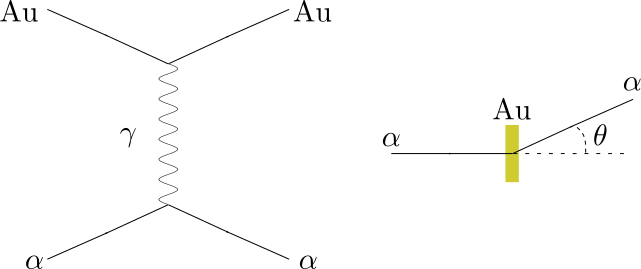
\includegraphics[scale=0.95]{scattering} %noinstiki
  \caption{Dispersi\'on de part\'\i culas $\alpha$ a trav\'es de una l\'amina de oro} %noinstiki
  \label{fig:sr} %noinstiki
\end{figure} %noinstiki<div id="fig:sr">Figura: Dispersi\'on</div>
%noinstiki![scattering](http://gfif.udea.edu.co/figfs/scattering.png)
%noinstiki

 
En general tendremos
\begin{equation}
\text{propagador:}\qquad \frac{1}{k^2-m^2},
\end{equation}
donde $k=(k_0,\mathbf{k})$




\chapter{Dirac Action}
\label{cha:dirac-action}


\section{Dirac's Action}
\label{sec:dirac-equation}
The Scrodinger equation can be written as
\begin{align}
    i\frac{\partial}{\partial t}\psi=\hat{H}_{S} \psi\,,  
\end{align}
where
\begin{align}
  \hat{H}_{S}=
\end{align}


In order to have a well defined probabilty in relativistic quantum mechanics it is necessary that Lagrangian be linear in the time derivative, in order to obtain the general Sccödinger equation:
\begin{align}
  i\frac{\partial}{\partial t}\psi=\hat{H} \psi\,,  
\end{align}
like the Scrödinger Lagrangian. However, this automatically imply that the Lagrangian will be also linear in the spacial derivatives. A pure scalar field cannot involve a Lorentz invariant term of only first derivatives (see eq.~\eqref{eq:nolor}). Therefore the proposed field must have some internal structure associated with some representation of the Lorentz Group. Therefore we build the Lagrangian for a field of several components
\begin{align}
  \psi=  \begin{pmatrix}
\psi_1\\
\psi_2\\
\vdots\\
\psi_n    
  \end{pmatrix}
\end{align}

\subsection{Lorentz transformation}

If the field is to describe the electron. it must have spin and in this way it must transform under some spin representation of the Lorentz Group
\begin{align}
  \psi(x)\to \psi'(x)=S(\Lambda)\psi\left(\Lambda^{-1}x\right)\,.
\end{align}
One possible invariant could be the term $\psi^\dagger(x)\psi(x)$. However, under a Lorentz transformation we should have $\psi^\dagger S^\dagger S\psi$. As we cannot assume that $S(\Lambda)$ is unitary, the solution is to define the \emph{adjoint} spinor
\begin{align}
  \overline{\psi}=\psi^\dagger b\,.
\end{align}
which transforms as
\begin{align}
  \overline{\psi}(x)\to  \overline{\psi}'(x)&=
{\psi'}^\dagger(x)b=
\psi^\dagger\left(\Lambda^{-1}x\right)S^\dagger(\Lambda)b\,,
\end{align}
and,

\begin{align}
  \overline{\psi}(x)\psi(x)\to  \overline{\psi}'(x)\psi'(x)&=
\psi^\dagger\left(\Lambda^{-1}x\right)S^\dagger(\Lambda)b S(\Lambda)\psi\left(\Lambda^{-1}x\right)
\end{align}
The condition that must be fulfilled for Lorentz invariance of the Action is 
\begin{align}
  \label{eq:ltrinscal}
  S^\dagger(\Lambda)bS(\Lambda)=&b\,,
\end{align}
and therefore, 
\begin{align}
  \overline{\psi}(x)\psi(x)\to  \overline{\psi}'(x)\psi'(x)&=
\overline{\psi}\left(\Lambda^{-1}x\right)\psi\left(\Lambda^{-1}x\right)\,,
\end{align}
and:
\begin{align}
  \overline{\psi}(x)\to  \overline{\psi}'(x)&=
\psi^\dagger\left(\Lambda^{-1}x\right)b S^{-1}(\Lambda)\nonumber\\
&=\overline{\psi}\left(\Lambda^{-1}x\right)S^{-1}(\Lambda)\,.
\end{align}


A Action with a Lagrangian term linear in the derivatives, could be Lorentz invariant if, taking into account:
 \begin{align}
   \overline{\psi}(x)\gamma^\mu\partial_\mu\psi(x)\to  \overline{\psi'}(x)\gamma^\mu\partial_\mu\psi'(x)&=
 \overline{\psi}_a\left(\Lambda^{-1}x\right)S^{-1}_{ab}(\Lambda)\gamma^\mu_{bc}{\left(\Lambda^{-1}\right)^\rho}_\mu\partial_\rho S_{cd}(\Lambda)\psi_d\left(\Lambda^{-1}x\right)\nonumber\\
   &=
\overline{\psi} \psi\left(\Lambda^{-1}x\right){\left(\Lambda^{-1}\right)^\rho}_\mu \left(S^{-1}(\Lambda)\gamma^\mu S(\Lambda)\right)\partial_\rho\psi\left(\Lambda^{-1}x\right)\nonumber\\
&=\overline{\psi}(x)\gamma^\mu\partial_\mu\psi(x)\,,
 \end{align}
if the following condition is satisfied:
\begin{align}
\label{eq:ltrincond}
  S^{-1}(\Lambda)\gamma^\mu S(\Lambda)={\Lambda^\mu}_\sigma\gamma^\sigma\,.
\end{align}




the most general Lagrangian for this field is
\begin{align}
   \mathcal{L}&=i \overline{\psi} \gamma^\mu\partial_\mu\psi-m\overline{\psi} \psi\,,
\end{align}
Where the coefficients have been already fixed by convenience. Since the Action is real, it is convenient to rewrite this as
\begin{align}
   \mathcal{L}&=i \overline{\psi} \gamma^\mu\partial_\mu\psi-m\overline{\psi} \psi\nonumber\\
&=-\frac{1}{2}\partial_\mu\left(i \overline{\psi} \gamma^\mu\psi\right)+i \overline{\psi} \gamma^\mu\partial_\mu\psi-m\overline{\psi} \psi\nonumber\\
  &=-\frac{i}{2}(\partial_\mu \overline{\psi}) \gamma^\mu\psi-\frac{i}{2} \overline{\psi} \gamma^\mu\partial_\mu\psi+i \overline{\psi} \gamma^\mu\partial_\mu\psi-m\overline{\psi} \psi\nonumber\\
  &=\frac{i}{2} \overline{\psi} \gamma^\mu\partial_\mu\psi-\frac{i}{2}(\partial_\mu \overline{\psi}) \gamma^\mu\psi-m\overline{\psi} \psi\,.
\end{align}
 
Para que este nuevo Lagrangiano sea real se requiere que,
\begin{align}
  \label{eq:185qft}
  b^\dagger&=b\nonumber\\
  b^2&=I\nonumber\\
  b \gamma_\mu^\dagger b&=\gamma_\mu
\end{align}
ya que
\begin{align*}
  \mathcal{L}^\dagger&=\left(\frac{i}{2}\psi^\dagger \gamma_\mu^\dagger b \partial_\mu\psi-\frac{i}{2}\partial_\mu\psi^\dagger \gamma_\mu^\dagger b\psi\right)-m\psi^\dagger  b \psi\\
  &=\left(\frac{i}{2}\psi^\dagger b^2 \gamma_\mu^\dagger b \partial_\mu\psi-\frac{i}{2}\partial_\mu\psi^\dagger b^2 \gamma_\mu^\dagger b\psi\right)-m\psi^\dagger b \psi\\
  &=\left(\frac{i}{2}\bar{\psi} b \gamma_\mu^\dagger b \partial_\mu\psi-\frac{i}{2}\partial_\mu\bar{\psi}b \gamma_\mu^\dagger b\psi\right)-m\bar{\psi} \psi\\
  &=\left(\frac{i}{2}\bar{\psi} \gamma_\mu \partial_\mu\psi-\frac{i}{2}\partial_\mu\bar{\psi}\gamma_\mu \psi\right)-m\bar{\psi} \psi
\end{align*}

\subsection{Corriente conservada y Lagrangiano de Dirac}
\label{sec:corriente-conservada}
De la ec.~\eqref{eq:197qft}
\begin{align}
  J^0&=\left[\frac{\partial\mathcal{L}}{\partial\left(\partial_0\psi\right)}\right]\delta\psi+\delta\overline{\psi}\left[\frac{\partial\mathcal{L}}{\partial\left(\partial_0\overline{\psi}\right)}\right]\nonumber\\
  &=i\overline{\psi} \gamma^0 \delta\psi
\end{align}
El Lagrangiano es invariante bajo transformaciones de fase globales, $U(1)$
\begin{equation}
  \psi\to\psi'=e^{-i\alpha}\psi\approx\psi-i\alpha\psi,
\end{equation}
de modo que
\begin{equation}
  \delta\psi=-i\alpha\psi.
\end{equation}
Por consiguiente
\begin{equation}
  J^0=\alpha\overline{\psi} \gamma^0 \psi 
\end{equation}
Para que $J^0$ pueda interpretarse como una densidad de probabilidad, se debe cumplir
\begin{equation}
  \label{eq:bgamma0}
  b \gamma^0=I
\end{equation}


La  densidad de corriente es
\begin{align}
  J^0&\propto \psi^\dagger\psi\,.
\end{align}
Que podemos interpretar como una densidad de probabilidad.

De la ec.~\eqref{eq:bgamma0}, ya que la inversa de es única:
\begin{align}
  b=\gamma^0\,.
\end{align}
 
$\overline{\psi}$ se define como la \emph{adjunta} de $\psi$:
 \begin{align}
   \overline{\psi}=\psi^\dagger\gamma^0\,.
 \end{align}

It is convenient at this point to summarize the properties for $\gamma^0$:
\begin{align}
  \label{eq:cft77}
  {\gamma^0}^\dagger=&\gamma^0 & \left(\gamma^0\right)^2=&1 & \gamma^0{\gamma^\mu}^\dagger\gamma^0=&\gamma^\mu\nonumber\\
 &&   S^\dagger(\Lambda)\gamma^0S(\Lambda)=&\gamma^0\,. &&
\end{align}



En general
\begin{align}
   J^\mu&\propto\left[\frac{\partial\mathcal{L}}{\partial\left(\partial_\mu\psi\right)}\right]\delta\psi+\delta\bar{\psi}\left[\frac{\partial\mathcal{L}}{\partial\left(\partial_\mu\bar{\psi}\right)}\right]\nonumber\\
   &\propto i\bar{\psi}\gamma^\mu(-i\alpha\psi)\nonumber\\
   &\propto i\bar{\psi}\gamma^\mu(-i\alpha\psi)\nonumber\\
   &=\bar{\psi}\gamma^\mu\psi
\end{align}
y
\begin{equation}
     J^\mu=\psi^\dagger b \gamma^\mu\psi\,.
\end{equation}

\subsection{Tensor momento-energía}
\label{sec:tens-momento-energi}
\begin{align}
  T^0_0&=\frac{\partial\mathcal{L}}{\partial\left(\partial_0\psi\right)}\partial_0\psi+\partial_0\bar{\psi}\frac{\partial\mathcal{L}}{\partial\left(\partial_0\bar{\psi}\right)}-\mathcal{L}\nonumber\\
  &=i\bar{\psi}\gamma^0\partial_0\psi-\mathcal{L}\nonumber\\
  &=-i\bar{\psi}\gamma^i\partial_i\psi+m\bar{\psi} \psi,\nonumber\\
  &=\bar{\psi}(\boldsymbol{\gamma}\cdot\mathbf{p}+m)\psi,\nonumber\\
  &=\psi^\dagger \gamma^0(\boldsymbol{\gamma}\cdot\mathbf{p}+m)\psi,\nonumber\\
  \label{eq:118qft}
  &=\psi^\dagger\hat{H} \psi,
\end{align}
donde
\begin{equation}
  \label{eq:denshal}
  \hat{H}= \gamma^0(\boldsymbol{\gamma}\cdot\mathbf{p}+m)
\end{equation}
la ecuación de Scröndinger de validez general es entonces:
\begin{equation}
  i\frac{\partial}{\partial t}\psi=\hat{H} \psi
\end{equation}
y, como en mecánica clásica usual
\begin{equation}
  \label{eq:99qft}
  \langle\hat{H}\rangle=\int \psi^\dagger\hat{H} \psi\,d^3x.
\end{equation}


Además
\begin{align}
    T^0_i&=\frac{\partial\mathcal{L}}{\partial\left(\partial_0\psi\right)}\partial_i\psi+\partial_i\bar{\psi}\frac{\partial\mathcal{L}}{\partial\left(\partial_0\bar{\psi}\right)}\nonumber\\
    &=i\bar{\psi}\gamma^0 \partial_i\psi\nonumber\\
    &=-\psi^\dagger(-i\partial_i)\psi
\end{align}
de modo que
\begin{equation}
  \langle\hat{\mathbf{p}}\rangle=\int\psi^\dagger\hat{\mathbf{p}}\psi\,d^3 x
\end{equation}
\subsection{Ecuaciones de Euler-Lagrange}
\label{sec:ecuaciones-de-euler}
Queremos que el Lagrangiano de lugar a la ecuación de Scröndinger de validez general
\begin{equation}
  \label{eq:grlsch}
  i\frac{\partial}{\partial t}\psi=\hat{H} \psi
\end{equation}
con el Hamiltoniano dado en la ec.~(\ref{eq:99qft}), que corresponde a un Lagrangiano de sólo derivadas de primer orden y covariante, en lugar del Hamiltoniano para el caso no relativista. 

De hecho, aplicando las ecuaciones de Euler-Lagrange para el campo $\bar{\psi}$ al Lagrangiano en ec.~(\ref{eq:100qft}) ,tenemos
\begin{align}
  \partial_\mu\left[\frac{\partial\mathcal{L}}{\partial\left(\partial_\mu\bar{\psi}\right)}\right]-\frac{\partial\mathcal{L}}{\partial\bar{\psi}}&=0\nonumber\\
  \frac{\partial\mathcal{L}}{\partial\bar{\psi}}&=0\nonumber\\
  \label{eq:114qftm}
  i\gamma^\mu\partial_\mu\psi-m\psi&=0.
\end{align}
Expandiendo
\begin{align*}
  i\gamma^0\partial_0\psi+i\gamma^i\partial_i\psi-m\psi&=0\\
  i\gamma^0\partial_0\psi-\boldsymbol{\gamma}\cdot(-i\boldsymbol{\nabla})\psi-m\psi&=0,\\
  i\gamma^0\partial_0\psi&=(\boldsymbol{\gamma}\cdot\hat{\mathbf{p}}+m)\psi,
\end{align*}
de donde
\begin{equation}
    i{\gamma^0}^2\frac{\partial}{\partial t}\psi=\gamma^0(\boldsymbol{\gamma}\cdot\mathbf{p}+m)\psi.
\end{equation}
 tenemos que
\begin{align}
  \label{eq:gamma02}
  \left(\gamma^0\right)^2=1.
\end{align}
De la ec.~(\ref{eq:denshal})
\begin{equation}
  \label{eq:186qft}
  \hat{H}= \gamma^0(\boldsymbol{\gamma}\cdot\mathbf{p}+m),
\end{equation}
A este punto, sólo nos queda por determinar los parámetros $\gamma^\mu$. 

La ec.~(\ref{eq:grlsch}) puede escribirse como
\begin{equation}
  \left(i\frac{\partial}{\partial t}-\hat{H}\right)\psi=0.
\end{equation}
El campo $\psi$ también debe satisfacer la ecuación de Klein-Gordon. Podemos derivar dicha ecuación aplicando el operador
\begin{equation*}
  \left(-i\frac{\partial}{\partial t}-\hat{H}\right)
\end{equation*}
De modo que, teniendo en cuenta que $\partial\hat H/\partial t=0$,
\begin{align}
  \label{eq:105qft}
 \left(-i\frac{\partial}{\partial t}-\hat{H}\right)\left(i\frac{\partial}{\partial t}-\hat{H}\right)\psi&=0\nonumber\\
 \left(-i\frac{\partial}{\partial t}-\hat{H}\right)\left(i\frac{\partial\psi}{\partial t}-\hat{H}\psi\right)&=0\nonumber\\
 \frac{\partial^2\psi}{\partial t^2}+i\left(\frac{\partial\hat{H}}{\partial t}\right)\psi
 +i\hat{H}\frac{\partial\psi}{\partial t}-i\hat{H}\frac{\partial\psi}{\partial t}+\hat{H}^2\psi&=0\nonumber\\
 \left(\frac{\partial^2}{\partial t^2}+\hat{H}^2\right)\psi&=0.
\end{align}
% 
De la ec.~(\ref{eq:186qft}), y usando la condición en ec.~(\ref{eq:gamma02}), tenemos
\begin{align}
\label{eq:106qft}
\hat{H}^2&=(\gamma_0\boldsymbol{\gamma}\cdot\mathbf{p}+\gamma_0\,m)(\gamma_0\boldsymbol{\gamma}\cdot\mathbf{p}+\gamma_0\,m)\nonumber\\
&=(\gamma_0\boldsymbol{\gamma}\cdot\mathbf{p})(\gamma_0\boldsymbol{\gamma}\cdot\mathbf{p})+m\gamma_0\boldsymbol{\gamma}\cdot\mathbf{p}\gamma_0+m\gamma_0^2\boldsymbol{\gamma}\cdot\mathbf{p}+m^2
\end{align}
Sea
\begin{align}
  \beta&=\gamma^0\nonumber\\
  \alpha^i&=\beta\gamma^i\nonumber\\
  \gamma^i&=\beta\alpha^i
\end{align}
\begin{align}
  \hat{H}^2&=(\boldsymbol{\alpha}\cdot\mathbf{p})(\boldsymbol{\alpha}\cdot\mathbf{p})
  +m\boldsymbol{\alpha}\cdot\mathbf{p}\beta+m\beta\boldsymbol{\alpha}\cdot\mathbf{p}+m^2\nonumber\\
  &=(\boldsymbol{\alpha}\cdot\mathbf{p})(\boldsymbol{\alpha}\cdot\mathbf{p})
  +m(\boldsymbol{\alpha}\beta+\beta\boldsymbol{\alpha})\cdot\mathbf{p}+m^2
\end{align}
Sea $A$ una matriz y $\theta$ en un escalar. Entonces tenemos la identidad
\begin{align}
  \label{eq:206qft}
  (\mathbf{A}\cdot\boldsymbol{\theta})^2=\sum_i {A^i}^2 {\theta^i}^2+\sum_{i\lt j}\left\{A^i,A^j  \right\}\theta^i \theta^j 
\end{align}
\begin{itemize}
\item \textbf{Demostración}
  \begin{align}
    \left[\left(\mathbf{A}\cdot\boldsymbol{\theta}\right)\right]_{\alpha\beta}
    =&\sum_{i j}\sum_\gamma A^i_{\alpha\gamma}\theta^iA^j_{\gamma\beta}\theta^j\nonumber\\    
    =&\sum_{i j}\theta^i\theta^j\sum_\gamma A^i_{\alpha\gamma}A^j_{\gamma\beta}\nonumber\\    
    =&\sum_\gamma \sum_{i j}\theta^i\theta^jA^i_{\alpha\gamma}A^j_{\gamma\beta}\nonumber\\    
    =&\sum_\gamma \left(\sum_{i}{\theta^i}^2A^i_{\alpha\gamma}A^i_{\gamma\beta}+\sum_{i<j}\theta^i\theta^jA^i_{\alpha\gamma}A^j_{\gamma\beta}+\sum_{i>j}\theta^i\theta^jA^i_{\alpha\gamma}A^j_{\gamma\beta}\right)\nonumber\\    
    =&\sum_\gamma \left(\sum_{i}{\theta^i}^2A^i_{\alpha\gamma}A^i_{\gamma\beta}+\sum_{i<j}\theta^i\theta^jA^i_{\alpha\gamma}A^j_{\gamma\beta}+\sum_{j>i}\theta^j\theta^iA^j_{\alpha\gamma}A^i_{\gamma\beta}\right)\nonumber\\    
    =&\sum_\gamma \left[\sum_{i}{\theta^i}^2A^i_{\alpha\gamma}A^i_{\gamma\beta}+\sum_{i<j}\theta^i\theta^j\left(A^i_{\alpha\gamma}A^j_{\gamma\beta}+A^j_{\alpha\gamma}A^i_{\gamma\beta}\right)\right]\nonumber\\    
    =&\left[\sum_{i}{\theta^i}^2\left(A^iA^i\right)_{\alpha\beta}+\sum_{i<j}\theta^i\theta^j\left\{ A^i,A^j\right\}_{\alpha\beta}\right]\nonumber\\    
    =&\left[\sum_{i}{\theta^i}^2{A^i}^2+\sum_{i<j}\theta^i\theta^j\left\{ A^i,A^j\right\}\right]_{\alpha\beta}\,.
  \end{align}

\end{itemize}
Entonces
\begin{align}
  \hat{H}^2=&\alpha_i^2p_i^2+\sum_{i\lt j}\left\{\alpha_i,\alpha_j\right\}p_i p_j+m(\alpha_i \beta+\beta\alpha_i)p_i+m^2
\end{align}
(suma sobre índices repetidos). Si
\begin{align}
  \label{eq:107qft}
  \alpha_i^2&=1\nonumber\\
  \left\{\alpha_i,\alpha_j\right\}&=0\qquad i\neq j\nonumber\\
  \alpha_i \beta+\beta\alpha_i&=0
\end{align}
\begin{equation}
  \hat{H}^2=-\boldsymbol{\nabla}^2+m^2
\end{equation}
y reemplazando en la ec.~\eqref{eq:105qft} llegamos a la ecuación de Klein-Gordon para $\psi$
\begin{align}
   \left(\frac{\partial^2}{\partial t^2}-\boldsymbol{\nabla}^2+m^2\right)\psi&=0\nonumber\\
   \left(\Box+m^2\right)\psi&=0
\end{align}
En términos de las matrices $\gamma^\mu$ las condiciones en ec.~\eqref{eq:107qft} son
\begin{align}
  \label{eq:108qft}
  \left({\gamma^0}\right)^2&=1\nonumber\\
  \left({\alpha^i}\right)^2=1\to\gamma^0\gamma^i \gamma^0\gamma^i=-\left({\gamma^i}\right)^2=1\to\left({\gamma^i}\right)^2&=-1\nonumber\\
  \gamma^i \gamma^0+\gamma^0\gamma^i=\left\{\gamma^i,\gamma^0\right\}&=0
\end{align}
De modo que
\begin{align}
  \label{eq:198qft}
\left\{\alpha^i,\alpha^j\right\}=\gamma^0\gamma^i \gamma^0\gamma^j+\gamma^0\gamma^j \gamma^0\gamma^i&=0\qquad i\neq j\nonumber\\
-\gamma^0\gamma^0\gamma^i \gamma^j-\gamma^0\gamma^0\gamma^j \gamma^i&=0\qquad i\neq j\nonumber\\
\gamma^i \gamma^j+\gamma^j \gamma^i&=0\qquad i\neq j\nonumber\\
\left\{\gamma^i,\gamma^j\right\}&=0\qquad i\neq j
\end{align}
Las ecuaciones \eqref{eq:108qft}\eqref{eq:198qft} pueden escribirse como
\begin{equation}
  \label{eq:109qft}
  \left\{\gamma^\mu,\gamma^\nu\right\}\equiv\gamma^\mu\gamma^\nu+\gamma^\nu\gamma^\mu=2g^{\mu\nu}\mathbf{1}
\end{equation}
donde
\begin{align}
  \gamma^\mu=(\gamma^0,\gamma^i)
\end{align}
Además, de la ec.~\eqref{eq:cft77}
\begin{equation}
  \label{eq:112qft}
   \gamma^0{\gamma^\mu}^\dagger \gamma^0=\gamma^\mu.
\end{equation}
Cualquier conjunto de matrices que satisfagan el álgebra en ec.~\eqref{eq:109qft} y la condición en ec.~\eqref{eq:112qft}, se conocen como matrices de Dirac. A $\psi$ se le llama espinor de Dirac.

En términos de la matrices $\gamma^\mu$, el Lagrangiano de Dirac y la ecuación de Dirac, son respectivamente de las ecs.~(\ref{eq:100qft}) y (\ref{eq:114qft})
\begin{equation}
  \label{eq:115qft}
  \mathcal{L}=\bar{\psi}\left(i\gamma^\mu\partial_\mu-m\right)\psi,
\end{equation}
\begin{equation}
  \label{eq:116qft}
  i\gamma^\mu\partial_\mu\psi-m\psi=0,
\end{equation}
donde
\begin{equation}
  \bar{\psi}=\psi^\dagger\gamma^0.
\end{equation}





\subsection{Propiedades de las matrices de Dirac}
\label{sec:propiedades-de-las}
De la ec.~(\ref{eq:112qft})
\begin{equation}
  {\gamma^\mu}^\dagger=\gamma^0\gamma^\mu\gamma^0\Rightarrow  
  \begin{cases}
    {\gamma^0}^\dagger=\gamma^0&\mu=0\\
    {\gamma^i}^\dagger=-{\gamma^0}^2\gamma^i=-\gamma^i&\mu=i
  \end{cases}.
\end{equation}
Definiendo
\begin{equation}
\label{eq:117qft}
  \gamma_5=i\gamma_0\gamma_1\gamma_2\gamma_3,
\end{equation}
entonces,
\begin{align}
  \gamma_5^2=&-\gamma_0\gamma_1\gamma_2\gamma_3\gamma_0\gamma_1\gamma_2\gamma_3\nonumber\\
  \gamma_5^2=&+\gamma_0^2\gamma_1\gamma_2\gamma_3\gamma_1\gamma_2\gamma_3\nonumber\\
  \gamma_5^2=&+\gamma_1\gamma_2\gamma_3\gamma_1\gamma_2\gamma_3\nonumber\\
  \gamma_5^2=&-\gamma_2\gamma_3\gamma_2\gamma_3\nonumber\\
  \gamma_5^2=&\gamma_2\gamma_2\gamma_3\gamma_3\nonumber\\
  \gamma_5^2=&\mathbf{1}\,.
\end{align}

\begin{equation}
  \gamma_5^2=\mathbf{1},
\end{equation}
Teniendo en cuenta que $\gamma_\mu^2\propto\mathbf{1}$ y conmuta con las demás matrices, tenemos por ejemplo
\begin{align}
  \gamma_5\gamma_3=&i\gamma_0\gamma_1\gamma_2\gamma_3^2=\gamma_3^2i\gamma_0\gamma_1\gamma_2=-\gamma_3i\gamma_0\gamma_1\gamma_2\gamma_3=-\gamma_3\gamma_5\nonumber\\
  \gamma_5\gamma_2=&-i\gamma_0\gamma_1\gamma_2^2\gamma_3=-\gamma_2^2i\gamma_0\gamma_1\gamma_3=-\gamma_2i\gamma_0\gamma_1\gamma_2\gamma_3=-\gamma_2\gamma_5\nonumber\\
  \gamma_5\gamma_1=&i\gamma_0\gamma_1^2\gamma_2\gamma_3=\gamma_1^2i\gamma_0\gamma_2\gamma_3=-\gamma_1i\gamma_0\gamma_1\gamma_2\gamma_3=-\gamma_1\gamma_5\nonumber\\
  \gamma_5\gamma_0=&i\gamma_0\gamma_1\gamma_2\gamma_3\gamma_0=-\gamma_0^2i\gamma_1\gamma_2\gamma_3=-\gamma_0\gamma_5\,.
\end{align}
De modo que
\begin{equation}
  \label{eq:218qft}
  \left\{\gamma_\mu,\gamma_5\right\}=0. 
\end{equation}
Expandiendo el anticonmutador tenemos
\begin{align}
  \gamma_\mu\gamma_5=-\gamma_5\gamma_\mu\nonumber\\
  \gamma_5\gamma_\mu\gamma_5=-\gamma_\mu\nonumber\\
\operatorname{Tr}\left(\gamma_5\gamma_\mu\gamma_5\right)=-\operatorname{Tr}\gamma_\mu\nonumber\\
\operatorname{Tr}\left(\gamma_5\gamma_5\gamma_\mu\right)=-\operatorname{Tr}\gamma_\mu\nonumber\\
\operatorname{Tr}\gamma_\mu=-\operatorname{Tr}\gamma_\mu,
\end{align}
y por consiguiente
\begin{equation}
  \operatorname{Tr}\gamma_\mu=0.
\end{equation}


De otro lado, si
\begin{equation}
  \tilde{\gamma_\mu}\equiv U\gamma_\mu U^\dagger,
\end{equation}
para alguna matriz unitaria $U$, entonces $\tilde{\gamma_\mu}$ corresponde a otra representación de álgebra de Dirac en ec.~(\ref{eq:109qft}), ya que
\begin{align}
  \left\{\tilde\gamma^\mu,\tilde\gamma^\nu\right\}&=\left\{U\gamma^\mu U^\dagger,U\gamma^\nu U^\dagger\right\}\nonumber\\
  &=U\left\{\gamma^\mu,\gamma^\nu\right\}U^\dagger\nonumber\\
  &=2g^{\mu\nu}UU^\dagger\nonumber\\
  &=2g^{\mu\nu}\mathbf{1}.
\end{align}
Claramente, la condición en ec.~(\ref{eq:112qft}) se mantiene para la nueva representación. Como $\gamma_0$ es hermítica, siempre es posible escoger una representación tal que $\tilde{\gamma_0}\equiv U\gamma_0U^\dagger$ sea diagonal. Como $\gamma_0^2=1$, sus entradas en la diagonal deben ser $\pm1$, y como $\operatorname{Tr}\tilde\gamma_0=0$, debe existir igual número de $+1$ que de $-1$. Por lo tanto la dimensión de $\gamma_0$ (y de $\gamma_\mu$) debe ser par: $2,4,\ldots$. Para un fermion sin masa
\begin{align}
  \mathcal{L}=i\psi^\dagger\gamma^0\gamma^0\partial_0\psi+i\psi^\dagger\gamma^0\gamma^i\partial_i\psi=i\psi^\dagger\partial_0\psi+i\psi^\dagger\alpha^i\partial_i\psi\,,
\end{align}
solo se requieren tres matrices $2\times 2$ que satisfacen
\begin{align}
  \left\{\alpha^i,\alpha^j\right\} =2\delta^{ij}\,,
\end{align}
y por lo tanto pueden identificarse con las tres matrices de Pauli. 
Como en general tenemos 4 matrices independientes, su dimensión mínima debe ser 4.

Como $\tilde\gamma^i=\gamma^0\gamma^i\gamma^0={\gamma^i}^\dagger=-\gamma^i$, podemos definir la \emph{representación de paridad}
\begin{align}
\label{eq:parityrep}
\tilde\gamma^0=&\gamma^0,\qquad\tilde\gamma^i=-\gamma^i\,,&\text{para}\qquad U=&\gamma^0   
\end{align}




\begin{inprogress}
  \subsection{Dirac representation}
The set of $4\times 4$ matrices
\begin{align}
  S^{\mu\nu}=\frac{i}{4}\left[\gamma^\mu,\gamma^\nu\right]\,,
\end{align}
also satisfy the commutations relations \eqref{eq:lrtalg}, and constitute a new matrix representation of the Lorentz Group. The subgroup of rotation group has the generators $S^{ij}$. We define the spin matrices:
\begin{align}
  \Sigma^i=\epsilon^{ijk}S_{jk}\,,
\end{align}
taking into account that
\begin{align}
  \gamma_0\gamma_i\gamma_5=-\epsilon_{0ijk}S^{jk}\,,
\end{align}
Taking th convention $\epsilon_{0ijk}=\epsilon_{ijk}$, we have
\begin{align}
  \Sigma_{i}=-\gamma_0\gamma_i\gamma_5\,.
\end{align}
With this form, it is easy to show that
\begin{align}
  \left\{\Sigma_i,\Sigma_j\right\}=2\delta_{ij}\,, 
\end{align}
so that 
\begin{align}
  \left[\frac{\Sigma^i}{2},\frac{\Sigma^j}{2} \right]=i\,\epsilon_{ijk}\frac{\Sigma^k}{2}
\end{align}
\end{inprogress}



\subsection{Lorentz invariance of the Dirac Action}
We need to satisfy the following conditions
\begin{align}
  S^{-1}(\Lambda) \gamma^\mu S(\Lambda)=&{\Lambda^\mu}_\nu\gamma^\nu\nonumber\\
  S^\dagger(\Lambda) \gamma^0 S(\Lambda)=&\gamma^0\qquad\text{or}\quad S^\dagger(\Lambda) \gamma^0= \gamma^0S^{-1}(\Lambda)\, .
\end{align}
We now set the notation
\begin{align}
\label{eq:lorentzrep}
  \Lambda=1+\xi_ib^i+\frac{1}{2}\theta_i\epsilon_{i j k}r^{jk}\,,
\end{align}
\begin{align}
 b^i=&-i J^{i0} & r^{jk}=-i J^{j k}\,.
\end{align}

In order to find a representation of the Lorentz Group in terms of the Dirac matrices we propose
  \begin{align}
    \label{eq:diraclorentzrep}
  S(\Lambda)=1+\xi_iB^i+\frac{1}{2}\theta_i\epsilon_{i j k}R^{jk}\,.
\end{align}
Instead of show the Lorentz invariance of the Dirac Action, we use the conditions derived from the invariance, to find a representation in terms of the Dirac matrices for $B^i$ and $R^{jk}$. As a consistency check, the resulting representation would satisfy the Lorentz algebra. In this way, by using eq.~\eqref{eq:lorentzrep} and \eqref{eq:diraclorentzrep}, we obtain from 
\begin{align}
  S^{-1}(\Lambda)\gamma^\mu S(\Lambda)={\Lambda^\mu}_\nu\gamma^\nu\,,
\end{align}
that
\begin{align}
  B^i=\frac{1}{2}\gamma^0\gamma^i\nonumber\\
  R^{jk}=&\frac{1}{2}\gamma^j\gamma^k\,,
\end{align}
which can be written in covariant form if we define
\begin{align}
  \mathcal{S}^{\mu\nu}=\frac{i}{4}\left[\gamma^\mu,\gamma^\nu\right]\,.
\end{align}
In fact, the six set of non-zero independently generators are
\begin{align}
  \mathcal{S}^{0i}=&\frac{i}{4}\left(\gamma^0\gamma^i-\gamma^i\gamma^0\right)=\frac{i}{2}\gamma^0\gamma^i= i B^i\nonumber\\
  \mathcal{S}^{i j}=&\frac{i}{4}\left(\gamma^i\gamma^j-\gamma^j\gamma^i\right)=\frac{i}{2}\gamma^i\gamma^j= i R^{i j}\,.
\end{align}
It is worth notices that in fact $\mathcal{S}^{\mu\nu}$ satisfy the Lorentz algebra, and therefore are the generators of the Lorentz group elements:
\begin{align}
  S(\Lambda)=&\exp\left(-i \omega_{\mu\nu}\frac{\mathcal{S}^{\mu\nu}}{2}\right)\nonumber\\
  \approx&1-\frac{i}{2} \omega_{\mu\nu}{\mathcal{S}^{\mu\nu}}\,.
\end{align}
Another consistency check is
\begin{align}
  S^\dagger(\Lambda)\gamma^0S(\Lambda)=&\gamma^0\,,
\end{align}
or equivalently
\begin{align}
S^\dagger(\Lambda)\gamma^0=&\gamma^0S^{-1}(\Lambda)\nonumber\\
\left(1+\frac{i}{2} \omega_{\mu\nu}{\mathcal{S}^{\mu\nu}}^\dagger \right)\gamma^0=&\gamma^0\left(1+\frac{i}{2} \omega_{\mu\nu}{\mathcal{S}^{\mu\nu}}\right)\nonumber\\
{\mathcal{S}^{\mu\nu}}^\dagger \gamma^0=&\gamma^0{\mathcal{S}^{\mu\nu}}\,.
\end{align}
Taking into account that
\begin{align}
  {\gamma^\mu}^\dagger{\gamma^\nu}^\dagger\gamma^0=\left(\gamma^0\right)^2{\gamma^\mu}^\dagger\left(\gamma^0\right)^2{\gamma^\nu}^\dagger\gamma^0=\gamma^0\gamma^\mu\gamma^\nu\,,
\end{align}
we have
\begin{align}
  {\mathcal{S}^{\mu\nu}}^\dagger \gamma^0=&-\frac{i}{4}\left[\gamma^\mu,\gamma^\nu\right]^\dagger\gamma^0\nonumber\\
=&-\frac{i}{4}\left[{\gamma^\nu}^\dagger,{\gamma^\mu}^\dagger\right]\gamma^0\nonumber\\
=&\frac{i}{4}\left[{\gamma^\mu}^\dagger,{\gamma^\nu}^\dagger\right]\gamma^0\nonumber\\
=&\frac{i}{4}\left[{\gamma^\mu},{\gamma^\nu}\right]\gamma^0\nonumber\\
=&\gamma^0\mathcal{S}^{\mu\nu}\nonumber\\
\end{align}


\subsection{Dirac's Lagrangian}
\label{sec:diracs-lagrangian}

Para una matriz de $n$ dimensiones existen $n^2$ matrices hermíticas (o anti--hermíticas) independientes. Si se sustrae la identidad quedan $n^2-1$ matrices hermíticas (o anti--hermíticas) independientes de traza nula. En el caso $n=2$ corresponden a las 3 matrices de Pauli. En el caso de la ecuación de Dirac se requieren 4 matrices independientes, por lo tanto deben ser matrices $4\times 4$. En efecto para $n=4$ existen 15 matrices independientes de traza nula dentro de las cuales podemos acomodar sin problemas las 4 $\gamma^\mu$. 

De \cite{Gross:1993}:
\begin{quote}
  All Dirac matrix elements will now be written in the form
  \begin{align}
    \overline{\psi}(x)\Gamma\psi(x)\,,
  \end{align}
where $\Gamma$ is a $4\times 4$ complex matrix. The most general such matrix can always be expanded in terms of 16 independent $4\times 4$ matrices multiplied by complex coefficients. In short the matrices $\Gamma$ can be regarded as a \emph{16--dimensional complex vector space} spanned by 16 matrices.

It is convenient to choose the 16 matrices, $\Gamma_i$, so that they have well defined transformation properties under the Lorentz Transformations. Since the $\gamma^\mu$'s have such properties, we are lead to choose the following 16 matrices for this basis:
\end{quote}


En la Tabla~\ref{tab:Gamma} se muestran las matrices de traza nula con sus propiedades de transformación bajo el Grupo de Lorentz. En la última se muestra el correspondiente escalar en el espacio de Dirac $\bar\psi\Gamma\psi$.
%instiki:
\begin{table} %noinstiki
  \centering %noinstiki
  \begin{tabular}{l|l|l|l} %noinstiki
Matriz $\Gamma$&Transformación&Número&Escalar en Dirac\\\hline{}
%instiki:
$\mathbf{1}$&Escalar (S)&1&$\bar\psi\psi$\\
%instiki:
$\gamma_5$&Pseudoescalar (P)&1&$\bar\psi\gamma_5\psi$\\
%instiki:
$\gamma_\mu$&Vector (V)&4&$\bar\psi\gamma_\mu\psi$\\
%instiki:
$\gamma_\mu\gamma_5$ &Vector axial (A)&4&$\bar\psi\gamma_\mu\gamma_5\psi$\\
%instiki:
$\sigma_{\mu\nu}=\frac{i}{2}\left[\gamma_\mu,\gamma_\nu\right]$&Tensor antisimétrico (T)&6&$\bar\psi\sigma_{\mu\nu}\psi$\\\hline{}
%instiki:
&&16&\\
  \end{tabular} %noinstiki
  \caption{Matrices $\Gamma_i$.} %noinstiki
\label{tab:Gamma} %noinstiki
\end{table} %noinstiki
%instiki:
Demostración
\begin{align}
J^\mu(x)\equiv  \bar\psi(x)\gamma^\mu\psi(x)\to&\bar\psi(\Lambda^{-1}x)S^{-1}(\Lambda)\gamma^\mu S(\Lambda)\psi(\Lambda^{-1}x) \nonumber\\
=&{\Lambda^\mu}_\nu\bar\psi(\Lambda^{-1}x) \gamma^\nu\psi(\Lambda^{-1}x) \nonumber\\
=&{\Lambda^\mu}_\nu J^\nu(\Lambda^{-1}x)\,.
\end{align}
In \cite{Gross:1993}: Problem 5.4: 
\begin{align}
  \overline{\psi}\gamma_5\psi\to\overline{\psi}S^{-1}(\Lambda)\gamma^5S(\Lambda)\psi =(\det\Lambda)\overline{\psi}\gamma_5\psi
\end{align}
The solution is in Appendix C. of Burgess book, by using
\begin{align}
  \gamma^5=\frac{i}{24}\epsilon_{\mu\nu\alpha\beta}\gamma^\mu\gamma^\nu\gamma^\alpha\gamma^\beta
\end{align}
and
\begin{align}
  \det \Lambda=\epsilon_{\mu\nu\alpha\beta}{\Lambda^\mu}_1{\Lambda^\nu}_2{\Lambda^\alpha}_3{\Lambda^\beta}_4\,.
\end{align}



\chapter{Soluciones a la ecuación de Dirac}
\label{cha:fermiones}
%instiki:
%instiki:***
%instiki:
%instiki:[[NotasFS|Tabla de Contenidos]]
%instiki:
%instiki:***
%instiki:
%instiki:* [Ecuaci\'on de Dirac](#ecuacion-de-dirac)
%instiki:
%instiki:* [Electrodin\'amica Cu\'antica](#electr-cuant)
%instiki:
%instiki:* [Cromodin\'amica Cu\'antica](#inter-fuert)
%instiki:
%instiki:* [Soluci\'on de part\'\i cula libre](#solucion-de-parti)
%instiki:
%instiki:***
%instiki:



\section{Fermiones quirales de cuatro componentes}
\label{sec:ferm-quir-de}

Sea
\begin{align}
  P_L\equiv&\frac{1-\gamma_5}{2}\nonumber\\
  P_R\equiv&\frac{1+\gamma_5}{2}\,.
\end{align}
Además
\begin{align}
  \psi_L\equiv P_L\psi\nonumber\\
  \psi_R\equiv P_R\psi\,.
\end{align}
Entonces
\begin{align}
  \psi=\psi_L+\psi_R\,.
\end{align}

Las matrices $P_{L,R}$ tienen las propiedades
\begin{align}
  P_L+P_R&=1 & P_{L,R}^2&=P_{L,R}P_{L,R}=P_{L,R}\nonumber\\
  P_L P_R&=0& P_{L,R}^\dagger&=P_{L,R}\,.
\end{align}
Usando la ec.~(\ref{eq:218qft})
\begin{align}
  P_{L,R}\gamma^\mu=\frac{1\mp\gamma_5}{2}\gamma^\mu=\gamma^\mu\frac{1\pm\gamma_5}{2}=\gamma^\mu P_{R,L}
\end{align}
Para escribir el Lagrangiano en término de los nuevos $\psi_{L,R}$ debemos tener en cuenta que
\begin{align}
  \overline{\psi_{L,R}}=(P_{L,R}\psi)^\dagger\gamma^0=\psi^\dagger P_{L,R}\gamma^0=\psi^\dagger\gamma^0P_{R,L}=\overline{\psi}P_{R,L}
\end{align}
\begin{align}
  \label{eq:221qft}
  \mathcal{L}=&i\overline{\psi}\gamma^\mu\partial_\mu\psi-m\overline{\psi}\psi\nonumber\\
  =&i\overline{\psi}(P_L+P_R)\gamma^\mu\partial_\mu\psi-m\overline{\psi}(P_L+P_R)\psi\nonumber\\
  =&i\overline{\psi}P_L\gamma^\mu\partial_\mu\psi+i\overline{\psi}P_R\gamma^\mu\partial_\mu\psi-m\overline{\psi}P_L\psi-m\overline{\psi}P_R\psi\nonumber\\
  =&i\overline{\psi}P_L P_L\gamma^\mu\partial_\mu\psi+i\overline{\psi}P_R P_R\gamma^\mu\partial_\mu\psi-m\overline{\psi}P_L P_L\psi-m\overline{\psi}P_R P_R\psi\nonumber\\
  =&i\overline{\psi}P_L\gamma^\mu\partial_\mu P_R\psi+i\overline{\psi}P_R\gamma^\mu\partial_\mu P_L\psi-m\overline{\psi}P_L P_L\psi-m\overline{\psi}P_R P_R\psi\nonumber\\
  =&i\overline{\psi_R}\gamma^\mu\partial_\mu\psi_R+i\overline{\psi_L}\gamma^\mu\partial_\mu\psi_L-m(\overline{\psi_R}\psi_L+\overline{\psi_L}\psi_R)\,.
\end{align}
En términos de espinores izquierdos y derechos de cuatro componentes la transformación de paridad 
\begin{align}
  \label{eq:220qft}
  t&\to t&\mathbf{x}&\to -\mathbf{x}&\psi_L(t,\mathbf{x})\to&\psi_R(t,-\mathbf{x}),& \psi_R(t,\mathbf{x})&\to\psi_L(t,-\mathbf{x})\nonumber\\
  \partial_0&\to \partial_0&\boldsymbol{\nabla}&\to -\boldsymbol{\nabla}&\psi_L(t,\mathbf{x})\to&\psi_R(t,-\mathbf{x}),& \psi_R(t,\mathbf{x})&\to\psi_L(t,-\mathbf{x})\,.
\end{align}
Además $\mathbf{L}=\mathbf{r}\times \mathbf{p}\to(-\mathbf{r})\times (-\mathbf{p})=\mathbf{L}$, y como $\gamma^\mu$ esta asociado al momento angular intrínsico, entonces también $\gamma^\mu\to\gamma^\mu$


Entonces la transformación de paridad da lugar a (sin tener en cuenta el cambio de argumento en los campos que desaparece en la integral de la Acción)
\begin{align}
  \overline{\psi_R}\gamma^\mu\partial_\mu\psi_R=\overline{\psi_R}\gamma^0\partial_0\psi_R+\overline{\psi_R}\boldsymbol{\gamma}\cdot\boldsymbol{\nabla}\psi_R 
\to&\overline{\psi_L}\gamma^0\partial_0\psi_L-\overline{\psi_L}\boldsymbol{\gamma}\cdot\boldsymbol{\nabla}\psi_L\nonumber\\
=&\overline{\psi_L}\gamma^0\partial_0\psi_L+\overline{\psi_L}\boldsymbol{\gamma}^\dagger\cdot\boldsymbol{\nabla}\psi_L\nonumber\\
=&\overline{\psi_L}\gamma^0\gamma^0\gamma^0\partial_0\psi_L+\overline{\psi_L}\gamma^0\boldsymbol{\gamma}\gamma^0\cdot\boldsymbol{\nabla}\psi_L\nonumber\\
=&\overline{\psi_L}\tilde\gamma^0\partial_0\psi_L+\overline{\psi_L}\tilde{\boldsymbol{\gamma}}\cdot\boldsymbol{\nabla}\psi_L\nonumber\\
=&\overline{\psi_L}\tilde\gamma^\mu\partial_\mu\psi_L\,.
\end{align}
Entonces
\begin{align}
   \mathcal{L}\to\mathcal{L}'=&i\overline{\psi_R}\tilde\gamma^\mu\partial_\mu\psi_R+i\overline{\psi_L}\tilde\gamma^\mu\partial_\mu\psi_L-m(\overline{\psi_R}\psi_L+\overline{\psi_L}\psi_R)\,,
\end{align}
donde $\tilde\gamma^\mu=U\gamma^\mu U^\dagger$, con $U=\gamma^0$. Como las dos representaciones dan lugar a la misma física, podemos decir que la Acción en términos de espinores $L,R$ de cuatro componentes es invariante bajo la transformación de paridad.

La existencia de ambos espinores $\psi_{L,R}$ garantizan que el Lagrangiano de Dirac es invariante bajo la transformación de paridad. 

La corriente de la electrodinámica cuántica en ec.~\eqref{eq:222qft} (o la de la cromodinámica cuántica, ec.~\eqref{eq:223qft}) conservan paridad ya que, siguiendo los mismos pasos que en la ec.~\eqref{eq:221qft}
\begin{align}
  \label{eq:224qft}
  \overline{\psi}\gamma^\mu\psi=\overline{\psi_L}\gamma^\mu\psi_L+\overline{\psi_R}\gamma^\mu\psi_R\to\overline{\psi_L}\tilde{\gamma}^\mu\psi_L+\overline{\psi_R}\tilde{\gamma}^\mu\psi_R\,.
\end{align}
Si para alguna partícula, como es el caso del neutrino, no existe la componente derecha, entonces la correspondiente interacción vectorial viola paridad y no puede tener ni interacciones electromagnéticas ni fuertes, es decir, no se acopla con el fotón o los gluones. Además dicha partícula no puede tener masa de Dirac. En el caso del neutrino esto se entiende pues al no tener carga eléctrica sólo requiere dos grados de libertad independientes.

De otro lado, si una determinada interacción, como es el caso de la interacción débil, solo participa la componente izquierda de la ec.~\eqref{eq:224qft}, está corresponde a una interacción del tipo
\begin{align}
  \overline{\psi}_L\gamma^\mu\psi_L&=\overline{\psi}P_R\gamma^\mu P_L\psi=\overline{\psi}\gamma^\mu P_L\psi\nonumber\\
  &=\overline{\psi}\gamma^\mu\left(\frac{1-\gamma_5}{2}\right)\psi\nonumber\\
  &=\tfrac{1}{2}\overline{\psi}\left(\gamma^\mu-\gamma^\mu\gamma_5\right)\psi\,,
\end{align}
que de acuerdo a la asignación en la Tabla corresponde a una corriente V--A. 

\subsection{Fermiones de Weyl}
\label{sec:fermiones-de-weyl}
%Weyl because $\psi^\dagger$ instead $\bar \psi$
Sea $\psi$ un campo que satisface una ecuaci\'on covariante de segundo orden. La parte cin\'etica del Lagrangiano sin t\'erminos de masa y sin t\'erminos de interacci\'on debe tener la forma 
\begin{equation}
\label{eq:98}
  \mathcal{L}=\frac{i}{2}\psi^\dagger a^\mu\partial_\mu\psi-\frac{i}{2}\partial_\mu\psi^\dagger {a^\mu}^\dagger\psi-m\psi^\dagger b\psi
\end{equation}
La Acci\'on debe ser real, de modo que el Lagrangiano tambi\'en. En efecto
\begin{align*}
  \mathcal{L}^\dagger&=\left(\frac{i}{2}\psi^\dagger a^\mu\partial_\mu\psi-\frac{i}{2}\partial_\mu\psi^\dagger {a^\mu}^\dagger\psi\right)^\dagger-m\psi^\dagger b^\dagger \psi\\
  &=\left(-\frac{i}{2}\partial^\mu\psi^\dagger a_\mu^\dagger \psi+\frac{i}{2}\psi^\dagger {a^\mu} \partial_\mu\psi\right)-m\psi^\dagger b^\dagger \psi\\
  &=\mathcal{L} \qquad \text{si }b^\dagger = b\,.
\end{align*}
Como al aplicar las ecuaciones de Euler-Lagrange a este Lagrangiano debemos obtener la ecuaci\'on de Scrh\"odinger
\begin{align}
i\frac{\partial}{\partial t}\psi=\widehat{H}\psi
\end{align}
con $\widehat{H}$ una funci\'on por determinar del operador $\hat{\mathbf{p}}$, entonces
\begin{align}
  a_\mu^\dagger=a_\mu
\end{align}

El Lagrangiano en ec.~(\ref{eq:98}) puede reescribirse como
\begin{align}
  \label{eq:197}
  \mathcal{L}&=\frac{i}{2}\psi^\dagger a^\mu\partial_\mu\psi-\frac{i}{2}\partial_\mu\left(\psi^\dagger a^\mu\psi\right)+\frac{i}{2}\psi^\dagger a^\mu\partial_\mu\psi-m\psi^\dagger b\psi\nonumber\\
  &=i \psi^\dagger a^\mu\partial_\mu\psi-\frac{i}{2}\partial_\mu\left(\psi^\dagger a^\mu\psi\right)-m\psi^\dagger b\psi\nonumber\\
  \mathcal{L}&=i \psi^\dagger a^\mu\partial_\mu\psi-m\psi^\dagger b\psi
\end{align}

Ahora utilizaremos el m\'etodo desarrollado en cap\'\i tulos anteriores para analizar el Lagrangiano. Calcularemos las ecuaciones de Euler-Lagrange, la corriente conservada y el tensor de momento-energ\'\i a.


\section{Soluciones a la ecuaci\'on de Dirac}
\label{sec:soluc-la-ecuac}

\subsection{Lagrangiano de Weyl}
\label{sec:lagrangiano-de-weyl}


En la ec.~\eqref{eq:118}, obtuvimos el Hamiltoniano en ec.~\eqref{eq:103}
\begin{equation}
  \hat{H}= \gamma_0(\boldsymbol{\gamma}\cdot\mathbf{p}+m)=\boldsymbol{\alpha}\cdot\mathbf{p}+\beta m\,.
\end{equation}
Una escogencia particular de las cuatro matrices $\gamma^\mu$, conocida como la representaci\'on de Weyl, o representaci\'on quiral, puede escribirse en t\'erminos de la matrices de Pauli. Escritas en bloques $2\times2$, tenemos
\begin{equation}
  \gamma^0=
  \begin{pmatrix}
    0&\sigma_0\\
    \sigma_0&0
  \end{pmatrix}\qquad
  \gamma_i=\begin{pmatrix}
    0&\sigma_i\\
    -\sigma_i&0
  \end{pmatrix}.
\end{equation}
Con $\sigma^0=1$. Con la matriz de tranformaci\'on
\begin{equation}
  U=\frac{1}{\sqrt{2}}
  \begin{pmatrix}
    1&1\\
    -1&1    
  \end{pmatrix}
\end{equation}
podemos obtener la representaci\'on de Dirac, tal que $U$ diagonaliza $\gamma^0$,
\begin{equation}
  \gamma^0=
  \begin{pmatrix}
    \sigma^0&0\\
    0&-\sigma^0
  \end{pmatrix}\qquad
  \gamma_i=\begin{pmatrix}
    0&\sigma_i\\
    -\sigma_i&0
  \end{pmatrix}.
\end{equation}
En adelante trabajaremos en la representaci\'on de Weyl que en forma compacta es
\begin{equation}
  \gamma^\mu=\begin{pmatrix}
    0&\sigma^\mu\\
    \bar{\sigma}^\mu & 0
  \end{pmatrix}
\end{equation}
donde
\begin{align}
  \sigma^\mu&=(\sigma^0,\sigma^1,\sigma^2,\sigma^3)\nonumber\\
  \bar{\sigma}^\mu&=(\sigma^0,-\sigma^1,-\sigma^2,-\sigma^3)\nonumber\\
\end{align}
Hemos escrito las matrices de Dirac en bloques $2\times2$, y es natural escribir similarmente las cuatro componentes del campo de Dirac como un par de campos de dos componentes
\begin{align}
  \psi=  \begin{pmatrix}
    \psi_L\\
    \psi_R    
  \end{pmatrix}=\begin{pmatrix}
    \psi_L\\
    0   
  \end{pmatrix}+\begin{pmatrix}
    0\\
    \psi_R    
  \end{pmatrix}
\end{align}
Donde $\psi_{L,R}$ son espinores de Weyl de dos componentes. En la representaci\'on de Weyl el Lagrangiano se puede escribir como
\begin{align}
\label{eq:200}
  \mathcal{L}=&i\bar{\psi}\gamma^\mu\partial_\mu\psi-m\bar{\psi}\psi\nonumber\\
  =&i\psi^\dagger \gamma^0\gamma^\mu\partial_\mu\psi-m\psi^\dagger \gamma^0 \psi\nonumber\\
  =&i\psi^\dagger  \begin{pmatrix}
    0 & 1\\
    1&0
  \end{pmatrix}
  \begin{pmatrix}
    0 &\sigma^\mu \\
    \bar{\sigma}^\mu&0
  \end{pmatrix}\partial_\mu\psi-m\psi^\dagger
  \begin{pmatrix}
    0 & 1\\
    1&0
  \end{pmatrix}\psi\nonumber\\
=&i\begin{pmatrix}
 \psi_L^\dagger & \psi_R^\dagger
\end{pmatrix}
 \begin{pmatrix}
   \bar{\sigma}^\mu &0\\
   0&\sigma^\mu
 \end{pmatrix} \begin{pmatrix}
   \partial_\mu\psi_L\\
   \partial_\mu\psi_R
 \end{pmatrix}-m
 \begin{pmatrix}
   \psi_L^\dagger&\psi_R^\dagger
 \end{pmatrix}
 \begin{pmatrix}
   0&1\\
   1&0
 \end{pmatrix}
 \begin{pmatrix}
   \psi_L\\ \psi_R
 \end{pmatrix}\nonumber\\
 =& i\psi_L^\dagger \bar{\sigma}^\mu\partial_\mu\psi_L+i\psi_R^\dagger \sigma^\mu\partial_\mu\psi_R
  -m(\psi_L^\dagger \psi_R+\psi_R^\dagger \psi_L)
\end{align}

\section{L\'\i mite no relativista en presencia de un campo electromagn\'etico}
\label{sec:limite-no-relat}
En el l\'\i mitie no relativista, la ecuaci\'on de Dirac en presencia de un campo electromagn\'etico (electrodin\'amica cu\'antica en la secci\'on \ref{sec:electr-cuant}) debe contener la ecuaci\'on de Scr\"odinger en presencia de un campo electromagn\'etico.
Combinando las ecuaciones \eqref{eq:203} tenemos
\begin{align}
  \label{eq:204}
  (i\partial_0- q A_0)(\psi_L+\psi_R)-{\sigma}^i(i\partial_i-q A_i)(\psi_L-\psi_R) -m(\psi_L+\psi_R) &=0\nonumber\\
  (i\partial_0-q A_0)(\psi_L-\psi_R)-{\sigma}^i(i\partial_i-q A_i)(\psi_L+\psi_R) +m(\psi_L-\psi_R) &=0
\end{align}
Esta forma es \'util porque de la soluci\'on de part\'\i culas libre esperamos que $\psi_L-\psi_R$ sea peque\~na. 
Como antes prongamos como soluci\'on
\begin{align}
  \psi_L=&u_L e^{-i p\cdot x} & \psi_R=&u_R e^{-i p\cdot x}
\end{align}

Para solucionar este sistema de ecuaciones acopladas definimos
\begin{align}
  \label{eq:216}
  \phi=e^{i m t}(\psi_L+\psi_R)&\Rightarrow(\psi_L+\psi_R)=e^{-i m t}\phi\nonumber\\
  \chi=e^{i m t}(\psi_L-\psi_R)&\Rightarrow(\psi_L-\psi_R)=e^{-i m t}\chi
\end{align}
donde
\begin{align}
\label{eq:260}
    \phi=&e^{i m t}(\psi_L+\psi_R)=e^{i m t}e^{-i (Et-\mathbf{p}\cdot x)}(u_L+u_R)=e^{i(m-E)t}e^{i\mathbf{p}\cdot x}(u_L+u_R)\nonumber\\
    \chi=&e^{i m t}(\psi_L-\psi_R)=e^{i m t}e^{-i (Et-\mathbf{p}\cdot x)}(u_L-u_R)=e^{i(m-E)t}e^{i\mathbf{p}\cdot x}(u_L-u_R)
\end{align}

Reemplazando~\eqref{eq:216} en eq.~\eqref{eq:204}
\begin{align}
  e^{-i m t}[m\phi+(i\partial_0- q A_0)\phi-{\sigma}^i(i\partial_i-q A_i)\chi-m\phi]  &=0\nonumber\\
  e^{-i m t}[m\chi+(i\partial_0-q A_0)\chi-{\sigma}^i(i\partial_i-q A_i)\phi+m\chi]  &=0
\end{align}
de donde
\begin{align}
  \label{eq:205}
  (i\partial_0- q A_0)\phi-{\sigma}^i(i\partial_i-q A_i)\chi  &=0\nonumber\\
  (i\partial_0-q A_0+2m)\chi-{\sigma}^i(i\partial_i-q A_i)\phi  &=0
\end{align}
Para una soluci\'on $\chi\propto e^{i(-Et-\mathbf{p}\cdot \mathbf{x})}$, dentro de un sistema at\'omico,  tenemos
\begin{equation}
  (i\partial_0-q A_0+2m)\chi=(E-q V+2m)\chi
\end{equation}
Para los potenciales de coulomb at\'omicos $qV=qA_0\sim10 eV$, y como $m\approx0.5\,$MeV para el electr\'on, entonces
\begin{equation}
  (i\partial_0-q A_0+2m)\chi\to(i\partial_0+2m)\chi
\end{equation}

de la ec.~\eqref{eq:260}  tenemos
\begin{align}
  (i\partial_0+2m)\chi=[(E-m)+2m]\chi
\end{align}
En el l\'\i mite no relativista de $|\mathbf{p}|\approx0$ ( estamos en la soluci\'on de energ\'\i a positiva), de la ec.~\eqref{eq:213} $E\approx+m$ y $E-m\approx0$, entonces
\begin{align}
  (i\partial_0+2m)\chi\approx2m\chi
\end{align}
Reemplazando en ec.~\eqref{eq:205}
\begin{equation}
  \chi=\frac{1}{2m}\sigma^i(i\partial_i-q A_i)\phi
\end{equation}
entonces
\begin{equation}
  i\frac{\partial}{\partial t}\phi=\widehat{H}\phi
\end{equation}
con
\begin{align}
  \widehat{H}\phi&= q A_0\phi+\sigma^i(i\partial_i-q A_i)\frac{1}{2m}\sigma^j(i\partial_j-q A_j)\phi  \nonumber\\
&=\frac{1}{2m}\sigma^i(i\partial_i-q A_i)\sigma^j(i\partial_j-q A_j)\phi+q A_0\phi\nonumber\\
  &=\frac{1}{2m}\sigma^i\sigma^j(-\partial_i\partial_j-i q(\partial_i A_j)-i qA_j\partial_i -i q A_i\partial_j+q^2 A_i A_j)\phi+q A_0\phi\nonumber\\
    &=\frac{1}{2m}\left[(-\sigma^i\sigma^j\partial_i\partial_j+q^2\sigma^i\sigma^jA_i A_j)\phi-i q \sigma^i\sigma^j (\partial_i A_j)\phi
    -i q\sigma^i\sigma^j A_j \partial_i\phi-i q\sigma^i\sigma^j A_i\partial_j\phi\right]+q A_0\phi\nonumber
\end{align}
Usando las propiedades de las matrices de Pauli en ecs.\eqref{eq:64} y la ec.\eqref{eq:206}, que  para $A^i=\sigma^i$ es
\begin{equation}
  (\boldsymbol{\sigma}\cdot\boldsymbol{\theta})^2=\sum_i\theta_i^2
\end{equation}
tenemos

\begin{align}
 \widehat{H}\phi &=\frac{1}{2m}\left\{[-(\boldsymbol{\sigma}\cdot\boldsymbol{\nabla})^2+q^2(\boldsymbol{\sigma}\cdot\mathbf{A})^2]\phi
    -i q\{\sigma^i,\sigma^j\} A_j \partial_i\phi-i q \sigma^i\sigma^j (\partial_i A_j)\phi\right\}+q A_0\phi\nonumber\\
    &=\frac{1}{2m}\left\{\sum_i[-\partial_i^2+q^2 A_i^2]\phi
     -2i q \delta_{ij} A_j \partial_i\phi-i q (i\epsilon_{ijk}\sigma^k+\delta_{ij})(\partial_i A_j) \phi\right\}+q A_0\phi\nonumber\\
    &=\frac{1}{2m}\left\{\sum_i[-\partial_i^2+q^2 A_i^2]\phi
     -2i q  A_i \partial_i\phi-i q(\partial_i A_i)\phi- q \sigma^k(\epsilon_{ijk}\partial_i A^j) \phi\right\}+q A_0\phi\nonumber
 \end{align}
Como
\begin{align}
  (i\boldsymbol{\nabla}+q\mathbf{A})^2\phi&=(i\partial_i-q A_i)(i\partial_i-q A_i)\phi\nonumber\\
  &=(-\partial_i\partial_i+q^2A_iA_i)\phi-i q(\partial_i A_i)\phi-i q A_i \partial_i\phi-i q A_i \partial_i\phi\nonumber\\
  &=\sum_i(-\partial_i^2+q^2A_i^2)\phi-2i q A_i \partial_i\phi-i q(\partial_i A_i)\phi
\end{align}
Entonces
\begin{align}
  \widehat{H}\phi&=\frac{1}{2m}\left\{(i\boldsymbol{\nabla}+q\mathbf{A})^2\phi
    -q \sigma^k(\boldsymbol{\nabla}\times\mathbf{A})_k \phi\right\}+q A_0\phi\nonumber\\
  &=\left[\frac{1}{2m}(i\boldsymbol{\nabla}+q \mathbf{A})^2+q A_0-\left(\frac{q\boldsymbol{\sigma}}{2m}\right)\cdot\mathbf{B}\right]\phi
\end{align}
%\left(\right)
En ausencia del campo electromagn\'etico recupermos la Ecuaci\'on de Scrh\"onger para una part\'\i cula libre como era de esperarse. Sin el \'ultimo t\'ermino $({q\boldsymbol{\sigma}}/{2m})\cdot\mathbf{B}$, ser\'\i a el Hamiltoniano de Scr\"odinger para una part\'\i cula cargada en presencia de un campo electromagn\'etico. El t\'ermino adicional es interpretado como la energ\'\i a en un campo magn\'etico, de un momento magn\'etico intr\'\i nseco asociado con un part\'\i cula de Dirac. Definimos entonces el momento magn\'etico intr\'\i nseco como ($q=-e$)
\begin{align}
  \boldsymbol{\mu}_e&=-\frac{e\boldsymbol{\sigma}}{2m}\nonumber\\
  &=-2\left(\frac{e}{2m}\right)\frac{\boldsymbol{\sigma}}{2}\nonumber\\
  &=-2\left(\frac{e\hbar}{2m}\right)\frac{\boldsymbol{\sigma}}{2}\nonumber\\
  &=-g_e\left(\frac{e\hbar}{2m}\right)\frac{\boldsymbol{\sigma}}{2}\nonumber\\
\end{align}
donde hemos recuperado el factor $\hbar$ y definido el \emph{factor--g} \cite{spin},  $g_e=2$. Se define el momento magn\'etico an\'omalo del electr\'on como
\begin{equation}
  a_e=\frac{g_e-2}{2}
\end{equation}
de modo que $a_e=0$. Sin embargo experimentalmente $a_e\sim10^{-3}$
\begin{equation}
  a_e=0.001\;159\;652\;1859(38)
\end{equation}
Despu\'es de la segunda cuantizaci\'on, se pueden realizar correcciones perturbativas al valor calculado anteriormente de $g_e$. Dicho c\'alculo ha sido realizado a cuarto orden en teor\'\i a de perturbaciones coincidiendo con el valor experimental hasta la d\'ecima cifra significativa. Este tipo de comprobaciones entre teor\'\i a y experimento ha llevado a considerar la Electrodin\'amica Cu\'antica (QCD) como la mejor teor\'\i a que se halla construido para describir la naturaleza. 




\section{Problemas}
\label{sec:problemas}
\begin{enumerate}%noinstiki
\item Calcule la dimensi\'on del campo $\psi$
\label{item:problemas5-1} %noinstiki
\item Demuestre que para una transformaci\'on $SU(3)_c$ global, los estados $B$ y $M$ en la ec.\eqref{eq:199} son invariantes. Es decir, son singletes de color (ver \cite{cottingham} \S16.2)
\label{item:problemas5-2} %noinstiki
\item Lagrangiano de Weyl.
  \begin{enumerate}
  \item Demuestre que $\psi_L^\dagger\bar{\sigma}^\mu\psi_L =-\psi_L\sigma^\mu\psi_L^\dagger$
  \item Definiendo $\xi=\psi_L$ y $\chi^\dagger=\psi_R$, demuestre que hasta derivadas totales
    \begin{equation}
      \mathcal{L}=i\xi^\dagger\bar{\sigma}^\mu\partial_\mu\xi+i\chi^\dagger\bar{\sigma}^\mu\partial_\mu\chi-m(\xi\chi+\xi^\dagger\chi^\dagger)
    \end{equation}
De modo que el Lagrangiano para un fermi\'on de Weyl, $\psi_W$, no masivo puede escribirse como
\begin{equation}
  \mathcal{L}=i\psi_W^\dagger\bar{\sigma}^\mu\partial_\mu\psi_W
\end{equation}
  \end{enumerate}
\label{item:problemas5-3}
\end{enumerate}%noinstiki

\section{Apéndices}


\section{Fermiones quirales de cuatro componentes}
\label{sec:ferm-quir-de}

Los fermiones izquierdos y derechos pueden ser escritos en terminos de espinores de Dirac como
\begin{align}
  \psi=\begin{pmatrix}
    \psi_L\\
    \psi_R
  \end{pmatrix}=
  \begin{pmatrix}
    \psi_L\\
    0    
  \end{pmatrix}+
  \begin{pmatrix}
    0\\
    \psi_R    
  \end{pmatrix}=&\widetilde{\psi}_L+\widetilde{\psi}_R
\end{align}
En la representaci\'on de Weyl
\begin{equation}
  \gamma_5=
  \begin{pmatrix}
    -1 & 0\\
    0 &1   
  \end{pmatrix}\,.
\end{equation}
Podemos definir
\begin{align}
  P_L\equiv&\frac{1-\gamma_5}{2}=
  \begin{pmatrix}
    1 & 0\\
    0 &0
  \end{pmatrix}\nonumber\\
  P_R\equiv&\frac{1+\gamma_5}{2}=
  \begin{pmatrix}
    0 & 0\\
    0 &1
  \end{pmatrix}\,.
\end{align}
De modo que
\begin{align}
  P_L\psi=&\begin{pmatrix}
    1 & 0\\
    0& 0    
  \end{pmatrix}
  \begin{pmatrix}
    \psi_L\\
    \psi_R
  \end{pmatrix}=
  \begin{pmatrix}
    \psi_L\\
    0
  \end{pmatrix}=\widetilde{\psi}_L\nonumber\\
  P_R\psi=&\widetilde{\psi}_R\,.
\end{align}
En adelante omitiremos las tildes sobre los espinores de Dirac $\widetilde{\psi}_{L,R}$.

Las matrices $P_{L,R}$ tienen las propiedades
\begin{align}
  P_L+P_R&=1 & P_{L,R}^2&=P_{L,R}P_{L,R}=P_{L,R}\nonumber\\
  P_L P_R&=0& P_{L,R}^\dagger&=P_{L,R}\,.
\end{align}
Usando la ec.~(\ref{eq:218})
\begin{align}
  P_{L,R}\gamma^\mu=\frac{1\mp\gamma_5}{2}\gamma^\mu=\gamma^\mu\frac{1\pm\gamma_5}{2}=\gamma^\mu P_{R,L}
\end{align}
Para escribir el Lagrangiano en t\'ermino de los nuevos $\psi_{L,R}$ debemos tener en cuenta que
\begin{align}
  \overline{\psi_{L,R}}=(P_{L,R}\psi)^\dagger\gamma^0=\psi^\dagger P_{L,R}\gamma^0=\psi^\dagger\gamma^0P_{R,L}=\overline{\psi}P_{R,L}
\end{align}
\begin{align}
  \label{eq:221}
  \mathcal{L}=&i\overline{\psi}\gamma^\mu\partial_\mu\psi-m\overline{\psi}\psi\nonumber\\
  =&i\overline{\psi}(P_L+P_R)\gamma^\mu\partial_\mu\psi-m\overline{\psi}(P_L+P_R)\psi\nonumber\\
  =&i\overline{\psi}P_L\gamma^\mu\partial_\mu\psi+i\overline{\psi}P_R\gamma^\mu\partial_\mu\psi-m\overline{\psi}P_L\psi-m\overline{\psi}P_R\psi\nonumber\\
  =&i\overline{\psi}P_L P_L\gamma^\mu\partial_\mu\psi+i\overline{\psi}P_R P_R\gamma^\mu\partial_\mu\psi-m\overline{\psi}P_L P_L\psi-m\overline{\psi}P_R P_R\psi\nonumber\\
  =&i\overline{\psi}P_L\gamma^\mu\partial_\mu P_R\psi+i\overline{\psi}P_R\gamma^\mu\partial_\mu P_L\psi-m\overline{\psi}P_L P_L\psi-m\overline{\psi}P_R P_R\psi\nonumber\\
  =&i\overline{\psi_R}\gamma^\mu\partial_\mu\psi_R+i\overline{\psi_L}\gamma^\mu\partial_\mu\psi_L-m(\overline{\psi_R}\psi_L+\overline{\psi_L}\psi_R)\,.
\end{align}
En t\'erminos de espinores de izquierdos y derechos de cuatro componentes la transformaci\'on de paridad 
\begin{align}
  \label{eq:220}
  t&\to t&\mathbf{x}&\to -\mathbf{x}&\psi_L\to&\psi_R,& \psi_R&\to\psi_L\,.
\end{align}
da lugar a
\begin{align}
   \mathcal{L}\to\mathcal{L}'=&i\overline{\psi_R}\tilde\gamma^\mu\partial_\mu\psi_R+i\overline{\psi_L}\tilde\gamma^\mu\partial_\mu\psi_L-m(\overline{\psi_R}\psi_L+\overline{\psi_L}\psi_R)\,,
\end{align}
donde $\tilde\gamma^\mu=U\gamma^\mu U^\dagger$, con $U=\gamma^0$. Como las dos representaciones dan lugar a la misma f\'\i sica, podemos decir que el LAgrangiano en t\'erminos de espinores $L,R$ de cuatro componentes es invariante bajo la transformaci\'on de paridad.

La existencia de ambos espinores $\psi_{L,R}$ garantizan que el Lagrangiano de Dirac es invariante bajo la transformaci\'on de paridad. 

La corriente de la electrodin\'amica cu\'antica en ec.~\eqref{eq:222} (o la de la cromodin\'amica cu\'antica, ec.~\eqref{eq:223}) conservan paridad ya que, siguiendo los mismos pasos que en la ec.~\eqref{eq:221}
\begin{align}
  \label{eq:224}
  \overline{\psi}\gamma^\mu\psi=\overline{\psi_L}\gamma^\mu\psi_L+\overline{\psi_R}\gamma^\mu\psi_R\,.
\end{align}
Si para alguna part\'\i cula, como es el caso del neutrino, no existe la componente derecha, entonces la correspondiente interacci\'on vectorial viola paridad y no puede tener interacciones electromagn\'eticas ni fuertes, es decir, no se acopla con el ft\'on o los gluones. Adem\'as dicha part\'\i cula no puede tener masa de Dirac. En el caso del neutrino esto se entiende pues al no tenr carga el\'ectrica s\'olo reuiere dos grados de libertad independientes.

De otro lado, si una determinada interacci\'on, como es el caso de la interacci\'on d\'ebil, solo participa la componente izquierda de la ec.~\eqref{eq:224}, est\'a corresponde a una interacci\'on del tipo
\begin{align}
  \overline{\psi}_L\gamma^\mu\psi_L&=\overline{\psi}P_R\gamma^\mu P_L\psi=\overline{\psi}\gamma^\mu P_L\psi\nonumber\\
  &=\overline{\psi}\gamma^\mu\left(\frac{1-\gamma_5}{2}\right)\psi\nonumber\\
  &=\tfrac{1}{2}\overline{\psi}\left(\gamma^\mu-\gamma^\mu\gamma_5\right)\psi\,,
\end{align}
que de acuerdo a la asignaci\'on en la Tabla corresponde a una corriente V--A. 





\subsection{Corriente conservada y Lagrangiano de Dirac}
\label{sec:corriente-conservada}
De la ec.~\eqref{eq:197}
\begin{align}
  J^0&=\left[\frac{\partial\mathcal{L}}{\partial\left(\partial_0\psi\right)}\right]\delta\psi+\delta\psi^\dagger\left[\frac{\partial\mathcal{L}}{\partial\left(\partial_0\psi^\dagger\right)}\right]\nonumber\\
  &=i\psi^\dagger a^0 \delta\psi
\end{align}
El Lagrangiano es invariante bajo transformaciones de fase globales, $U(1)$
\begin{equation}
  \psi\to\psi'=e^{-i\alpha}\psi\approx\psi-i\alpha\psi,
\end{equation}
de modo que
\begin{equation}
  \delta\psi=-i\alpha\psi.
\end{equation}
Por consiguiente
\begin{equation}
  J^0=\alpha\psi^\dagger a^0 \psi 
\end{equation}
Para que $J^0$ pueda interpretarse como una densidad de probabilidad, debemos redefinir el Lagrangiano en ec.~\eqref{eq:98} como
\begin{equation}
  \label{eq:113}
    \mathcal{L}=\frac{i}{2}\bar{\psi} \gamma^\mu\partial_\mu\psi-\frac{i}{2}\partial_\mu\bar \psi \gamma^\mu\psi-m\bar{\psi} b\psi,
\end{equation}
tal que
\begin{equation}
  \bar{\psi}=\psi^\dagger c,
\end{equation}
con
\begin{equation}
  c \gamma^0=I
\end{equation}
Para que este nuevo Lagrangiano sea real se requiere que,
\begin{align}
  c^2&=I\nonumber\\
  c \gamma_\mu^\dagger c&=\gamma_\mu\nonumber\\
  \label{eq:110}
  c b^\dagger c&=b
\end{align}
ya que
\begin{align*}
  \mathcal{L}^\dagger&=\left(\frac{i}{2}\psi^\dagger \gamma_\mu^\dagger c \partial_\mu\psi-\frac{i}{2}\partial_\mu\psi^\dagger \gamma_\mu^\dagger c\psi\right)-m\psi^\dagger b^\dagger c \psi\\
  &=\left(\frac{i}{2}\psi^\dagger c^2 \gamma_\mu^\dagger c \partial_\mu\psi-\frac{i}{2}\partial_\mu\psi^\dagger c^2 \gamma_\mu^\dagger c\psi\right)-m\psi^\dagger c^2 b^\dagger c \psi\\
  &=\left(\frac{i}{2}\bar{\psi} c \gamma_\mu^\dagger c \partial_\mu\psi-\frac{i}{2}\partial_\mu\bar{\psi}c \gamma_\mu^\dagger c\psi\right)-m\bar{\psi}c b^\dagger c \psi\\
  &=\left(\frac{i}{2}\bar{\psi} \gamma_\mu \partial_\mu\psi-\frac{i}{2}\partial_\mu\bar{\psi}\gamma_\mu \psi\right)-m\bar{\psi}b \psi
\end{align*}
Sin perdida de generalidad podemos hacer $b=I$, y
\begin{equation}
  \label{eq:100}
    \mathcal{L}=i\bar{\psi} \gamma^\mu\partial_\mu\psi-m\bar{\psi} \psi,
\end{equation}
La nueva corriente conservada contiene
\begin{align}
  J^0&\propto\left[\frac{\partial\mathcal{L}}{\partial\left(\partial_0\psi\right)}\right]\delta\psi+\delta\bar{\psi}\left[\frac{\partial\mathcal{L}}{\partial\left(\partial_0\bar{\psi}\right)}\right]\nonumber\\
  &=\bar{\psi}\gamma^0\psi\nonumber\\
  &=\psi^\dagger c \gamma^0 \psi\nonumber\\
  &=\psi^\dagger\psi
\end{align}
Que podemos interpretar como una densidad de probabilidad. $\bar \psi$ se define como la \emph{adjunta} de $\psi$.

En general
\begin{align}
   J^\mu&\propto\left[\frac{\partial\mathcal{L}}{\partial\left(\partial_\mu\psi\right)}\right]\delta\psi+\delta\bar{\psi}\left[\frac{\partial\mathcal{L}}{\partial\left(\partial_\mu\bar{\psi}\right)}\right]\nonumber\\
   &\propto i\bar{\psi}\gamma^\mu(-i\alpha\psi)\nonumber\\
   &\propto i\bar{\psi}\gamma^\mu(-i\alpha\psi)\nonumber\\
   &=\bar{\psi}\gamma^\mu\psi
\end{align}
y
\begin{equation}
     J^\mu=\psi^\dagger c \gamma^\mu\Psi
\end{equation}

\subsection{Tensor momento-energ\'\i a}
\label{sec:tens-momento-energi}
\begin{align}
  T^0_0&=\frac{\partial\mathcal{L}}{\partial\left(\partial_0\psi\right)}\partial_0\psi+\partial_0\bar{\psi}\frac{\partial\mathcal{L}}{\partial\left(\partial_0\bar{\psi}\right)}-\mathcal{L}\nonumber\\
  &=i\bar{\psi}\gamma^0\partial_0\psi-\mathcal{L}\nonumber\\
  &=-i\bar{\psi}\gamma^i\partial_i\psi+m\bar{\psi} \psi,\nonumber\\
  &=\bar{\psi}(\boldsymbol{\gamma}\cdot\mathbf{p}+m)\psi,\nonumber\\
  &=\psi^\dagger c(\boldsymbol{\gamma}\cdot\mathbf{p}+m)\psi,\nonumber\\
  \label{eq:118}
  &=\psi^\dagger\hat{H} \psi,
\end{align}
donde
\begin{equation}
  \label{eq:101}
  \hat{H}= c(\boldsymbol{\gamma}\cdot\mathbf{p}+m)
\end{equation}
y, como en mec\'anica cl\'asica usual
\begin{equation}
  \label{eq:99}
  \langle\hat{H}\rangle=\int \psi^\dagger\hat{H} \psi\,d^3x.
\end{equation}
Adem\'as
\begin{align}
    T^0_i&=\frac{\partial\mathcal{L}}{\partial\left(\partial_0\psi\right)}\partial_i\psi+\partial_i\bar{\psi}\frac{\partial\mathcal{L}}{\partial\left(\partial_0\bar{\psi}\right)}\nonumber\\
    &=i\bar{\psi}\gamma^0 \partial_i\psi\nonumber\\
    &=-\psi^\dagger(-i\partial_i)\psi
\end{align}
de modo que
\begin{equation}
  \langle\hat{\mathbf{p}}\rangle=\int\psi^\dagger\hat{\mathbf{p}}\psi\,d^3 x
\end{equation}
\subsection{Ecuaciones de Euler-Lagrange}
\label{sec:ecuaciones-de-euler}
Queremos que el Lagrangiano de lugar a la ecuaci\'on de Scr\"ondinger de validez general
\begin{equation}
  \label{eq:102}
  i\frac{\partial}{\partial t}\psi=\hat{H} \psi
\end{equation}
con el Hamiltoniano dado en la ec.~(\ref{eq:99}), que corresponde a un Lagrangiano de s\'olo derivadas de primer orden y covariante, en lugar del Hamiltoniano para el caso no relativista. 

De hecho, aplicando las ecuaciones de Euler-Lagrange para el campo $\bar{\psi}$ al Lagrangiano en ec.~(\ref{eq:100}) ,tenemos
\begin{align}
  \partial_\mu\left[\frac{\partial\mathcal{L}}{\partial\left(\partial_\mu\bar{\psi}\right)}\right]-\frac{\partial\mathcal{L}}{\partial\bar{\psi}}&=0\nonumber\\
  \frac{\partial\mathcal{L}}{\partial\bar{\psi}}&=0\nonumber\\
  \label{eq:114}
  i\gamma^\mu\partial_\mu\psi-m\psi&=0.
\end{align}
Expandiendo
\begin{align*}
  i\gamma^0\partial_0\psi+i\gamma^i\partial_i\psi-m\psi&=0\\
  i\gamma^0\partial_0\psi-\boldsymbol{\gamma}\cdot(-i\boldsymbol{\nabla})\psi-m\psi&=0,\\
  i\gamma^0\partial_0\psi&=(\boldsymbol{\gamma}\cdot\hat{\mathbf{p}}+m)\psi,
\end{align*}
de donde
\begin{equation}
    i{\gamma^0}^2\frac{\partial}{\partial t}\psi=\gamma^0(\boldsymbol{\gamma}\cdot\mathbf{p}+m)\psi.
\end{equation}
Comparando con ecs.~(\ref{eq:102}) y (\ref{eq:101}), tenemos que
\begin{align}
  c=\gamma^0\nonumber\\
  \label{eq:104}
  {\gamma^0}^2=1.
\end{align}
De la ec.~(\ref{eq:101})
\begin{equation}
  \label{eq:103}
  \hat{H}= \gamma^0(\boldsymbol{\gamma}\cdot\mathbf{p}+m),
\end{equation}
y de la ec.~\eqref{eq:110}
\begin{equation}
  \label{eq:111}
  \gamma^0{\gamma^\mu}^\dagger \gamma^0=\gamma^\mu.
\end{equation}
A este punto, s\'olo nos queda por determinar los par\'ametros $\gamma^\mu$. 

La ec.~(\ref{eq:102}) puede escribirse como
\begin{equation}
  \left(i\frac{\partial}{\partial t}-\hat{H}\right)\psi=0.
\end{equation}
El campo $\psi$ tambi\'en debe satisfacer la ecuaci\'on de Klein-Gordon. Podemos derivar dicha ecuaci\'on aplicando el operador
\begin{equation*}
  \left(-i\frac{\partial}{\partial t}-\hat{H}\right)
\end{equation*}
De modo que, teniendo en cuenta que $\partial\hat H/\partial t=0$,
\begin{align}
  \label{eq:105}
 \left(-i\frac{\partial}{\partial t}-\hat{H}\right)\left(i\frac{\partial}{\partial t}-\hat{H}\right)\psi&=0\nonumber\\
 \left(-i\frac{\partial}{\partial t}-\hat{H}\right)\left(i\frac{\partial\psi}{\partial t}-\hat{H}\psi\right)&=0\nonumber\\
 \frac{\partial^2\psi}{\partial t^2}+i\left(\frac{\partial\hat{H}}{\partial t}\right)\psi
 +i\hat{H}\frac{\partial\psi}{\partial t}-i\hat{H}\frac{\partial\psi}{\partial t}+\hat{H}^2\psi&=0\nonumber\\
 \left(\frac{\partial^2}{\partial t^2}+\hat{H}^2\right)\psi&=0.
\end{align}
% 
De la ec.~(\ref{eq:103}), y usando la condici\'on en ec.~(\ref{eq:104}), tenemos
\begin{align}
\label{eq:106}
\hat{H}^2&=(\gamma_0\boldsymbol{\gamma}\cdot\mathbf{p}+\gamma_0\,m)(\gamma_0\boldsymbol{\gamma}\cdot\mathbf{p}+\gamma_0\,m)\nonumber\\
&=(\gamma_0\boldsymbol{\gamma}\cdot\mathbf{p})(\gamma_0\boldsymbol{\gamma}\cdot\mathbf{p})+m\gamma_0\boldsymbol{\gamma}\cdot\mathbf{p}\gamma_0+m\gamma_0^2\boldsymbol{\gamma}\cdot\mathbf{p}+m^2
\end{align}
Sea
\begin{align}
  \beta&=\gamma^0\nonumber\\
  \alpha^i&=\beta\gamma^i\nonumber\\
  \gamma^i&=\beta\alpha^i
\end{align}
\begin{align}
  \hat{H}^2&=(\boldsymbol{\alpha}\cdot\mathbf{p})(\boldsymbol{\alpha}\cdot\mathbf{p})
  +m\boldsymbol{\alpha}\cdot\mathbf{p}\beta+m\beta\boldsymbol{\alpha}\cdot\mathbf{p}+m^2\nonumber\\
  &=(\boldsymbol{\alpha}\cdot\mathbf{p})(\boldsymbol{\alpha}\cdot\mathbf{p})
  +m(\boldsymbol{\alpha}\beta+\beta\boldsymbol{\alpha})\cdot\mathbf{p}+m^2
\end{align}
Sea $A$ una matriz y $\theta$ en un escalar. Entonces tenemos la identidad
\begin{align}
  \label{eq:206}
  (\mathbf{A}\cdot\boldsymbol{\theta})^2=\sum_i {A^i}^2 {\theta^i}^2+\sum_{i\lt j}\left\{A^i,A^j  \right\}\theta^i \theta^j 
\end{align}
Entonces
\begin{align}
  \hat{H}^2=&\alpha_i^2p_i^2+\sum_{i\lt j}\left\{\alpha_i,\alpha_j\right\}p_i p_j+m(\alpha_i \beta+\beta\alpha_i)p_i+m^2
\end{align}
(suma sobre \'\i ndices repetidos). Si
\begin{align}
  \label{eq:107}
  \alpha_i^2&=1\nonumber\\
  \left\{\alpha_i,\alpha_j\right\}&=0\qquad i\neq j\nonumber\\
  \alpha_i \beta+\beta\alpha_i&=0
\end{align}
\begin{equation}
  \hat{H}^2=-\boldsymbol{\nabla}^2+m^2
\end{equation}
y reemplazando en la ec.~\eqref{eq:105} llegamos a la ecuaci\'on de Klein-Gordon para $\psi$
\begin{align}
   \left(\frac{\partial^2}{\partial t^2}-\boldsymbol{\nabla}^2+m^2\right)\psi&=0\nonumber\\
   \left(\Box+m^2\right)\psi&=0
\end{align}
En t\'erminos de las matrices $\gamma^\mu$ las condiciones en ec.~\eqref{eq:107} son
\begin{align}
  \label{eq:108}
  {\gamma^0}^2&=1\nonumber\\
  {\alpha^i}^2=1\to\gamma^0\gamma^i \gamma^0\gamma^i=-{\gamma^i}^2=1\to{\gamma^i}^2&=-1\nonumber\\
  \gamma^i \gamma^0+\gamma^0\gamma^i=\left\{\gamma^i,\gamma^0\right\}&=0
\end{align}
De modo que
\begin{align}
  \label{eq:198}
\left\{\alpha^i,\alpha^j\right\}=\gamma^0\gamma^i \gamma^0\gamma^j+\gamma^0\gamma^j \gamma^0\gamma^j&=0\qquad i\neq j\nonumber\\
-\gamma^0\gamma^0\gamma^i \gamma^j-\gamma^0\gamma^0\gamma^j \gamma^j&=0\qquad i\neq j\nonumber\\
\gamma^i \gamma^j+\gamma^j \gamma^j&=0\qquad i\neq j\nonumber\\
\left\{\gamma^i,\gamma^j\right\}&=0\qquad i\neq j
\end{align}
Las ecuaciones \eqref{eq:108}\eqref{eq:198} pueden escribirse como
\begin{equation}
  \label{eq:109}
  \left\{\gamma^\mu,\gamma^\nu\right\}\equiv\gamma^\mu\gamma^\nu+\gamma^\nu\gamma^\mu=2g^{\mu\nu}.
\end{equation}
donde
\begin{align}
  \gamma^\mu=(\gamma^0,\gamma^i)
\end{align}
Adem\'as, de la ec.~\eqref{eq:111},
\begin{equation}
  \label{eq:112}
   \gamma^0{\gamma^\mu}^\dagger \gamma^0=\gamma^\mu.
\end{equation}
Cualquier conjunto de matrices que satisfagan el \'algebra en ec.~\eqref{eq:109} y la condici\'on en ec.~\eqref{eq:112}, se conocen como matrices de Dirac. A $\psi$ se le llama espinor de Dirac.

En t\'erminos de la matrices $\gamma^\mu$, el Lagrangiano de Dirac y la ecuaci\'on de Dirac, son respectivamente de las ecs.~(\ref{eq:100}) y (\ref{eq:114})
\begin{equation}
  \label{eq:115}
  \mathcal{L}=\bar{\psi}\left(i\gamma^\mu\partial_\mu-m\right)\psi,
\end{equation}
\begin{equation}
  \label{eq:116}
  i\gamma^\mu\partial_\mu\psi-m\psi=0,
\end{equation}
donde
\begin{equation}
  \bar{\psi}=\psi^\dagger\gamma^0.
\end{equation}

\subsection{Propiedades de las matrices de Dirac}
\label{sec:propiedades-de-las}
De la ec.~(\ref{eq:112})
\begin{equation}
  {\gamma^\mu}^\dagger=\gamma^0\gamma^\mu\gamma^0\Rightarrow  
  \begin{cases}
    {\gamma^0}^\dagger=\gamma^0&\mu=0\\
    {\gamma^i}^\dagger=-{\gamma^0}^2\gamma^i=-\gamma^i&\mu=i
  \end{cases}.
\end{equation}
Definiendo
\begin{equation}
\label{eq:117}
  \gamma_5=i\gamma_0\gamma_1\gamma_2\gamma_3,
\end{equation}
entonces, 
\begin{equation}
  \gamma_5^2=\mathbf{1},
\end{equation}
Teniendo en cuenta que $\gamma_\mu^2\propto\mathbf{1}$ y conmuta con las dem\'as matrices, tenemos por ejemplo
\begin{align}
  \gamma_5\gamma_3=&i\gamma_0\gamma_1\gamma_2\gamma_3^2=\gamma_3^2i\gamma_0\gamma_1\gamma_2=-\gamma_3i\gamma_0\gamma_1\gamma_2\gamma_3=-\gamma_3\gamma_5\nonumber\\
  \gamma_5\gamma_2=&-i\gamma_0\gamma_1\gamma_2^2\gamma_3=-\gamma_2^2i\gamma_0\gamma_1\gamma_3=-\gamma_2i\gamma_0\gamma_1\gamma_2\gamma_3=-\gamma_2\gamma_5\nonumber\\
  \gamma_5\gamma_1=&i\gamma_0\gamma_1^2\gamma_2\gamma_3=\gamma_1^2i\gamma_0\gamma_2\gamma_3=-\gamma_1i\gamma_0\gamma_1\gamma_2\gamma_3=-\gamma_1\gamma_5\nonumber\\
  \gamma_5\gamma_0=&i\gamma_0\gamma_1\gamma_2\gamma_3\gamma_0=-\gamma_0^2i\gamma_1\gamma_2\gamma_3=-\gamma_0\gamma_5\,.
\end{align}
De modo que
\begin{equation}
  \label{eq:218}
  \left\{\gamma_\mu,\gamma_5\right\}=0. 
\end{equation}
Expandiendo el anticonmutador tenemos
\begin{align}
  \gamma_\mu\gamma_5=-\gamma_5\gamma_\mu\nonumber\\
  \gamma_5\gamma_\mu\gamma_5=-\gamma_\mu\nonumber\\
\operatorname{Tr}\left(\gamma_5\gamma_\mu\gamma_5\right)=-\operatorname{Tr}\gamma_\mu\nonumber\\
\operatorname{Tr}\left(\gamma_5\gamma_5\gamma_\mu\right)=-\operatorname{Tr}\gamma_\mu\nonumber\\
\operatorname{Tr}\gamma_\mu=-\operatorname{Tr}\gamma_\mu,
\end{align}
y por consiguiente
\begin{equation}
  \operatorname{Tr}\gamma_\mu=0.
\end{equation}
Si
\begin{equation}
  \tilde{\gamma_\mu}\equiv U\gamma_\mu U^\dagger,
\end{equation}
para alguna matriz unitaria $U$, entonces $\tilde{\gamma_\mu}$ corresponde a otra representaci\'on de \'algebra de Dirac en ec.~(\ref{eq:109}), ya que
\begin{align}
  \left\{\tilde\gamma^\mu,\tilde\gamma^\nu\right\}&=\left\{U\gamma^\mu U^\dagger,U\gamma^\nu U^\dagger\right\}\nonumber\\
  &=U\left\{\gamma^\mu,\gamma^\nu\right\}U^\dagger\nonumber\\
  &=2g^{\mu\nu}UU^\dagger\nonumber\\
  &=2g^{\mu\nu}.
\end{align}
Claramente, la condici\'on en ec.~(\ref{eq:112}) se mantiene para la nueva representaci\'on. Como $\gamma_0$ es herm\'\i tica, siempre es posible escoger una representaci\'on tal que $\tilde{\gamma_0}\equiv U\gamma_0U^\dagger$ sea diagonal. Como $\gamma_0^2=1$, sus entradas en la diagonal deben ser $\pm1$, y como $\operatorname{Tr}\tilde\gamma_0=0$, debe existir igual n\'umero de $+1$ que de $-1$. Por lo tanto la dimensi\'on de $\gamma_0$ (y de $\gamma_\mu$) debe ser par: $2,4,\ldots$. 

Si $U=\gamma^0$, entonces $\tilde\gamma^0=\gamma^0$ y $\tilde\gamma^i=-\gamma^i$. 

Para una matriz de $n$ dimensiones existen $n^2$ matrices herm\'\i ticas (o anti--herm\'\i ticas) independientes. Si se sustrae la identidad quedan $n^2-1$ matrices herm\'\i ticas (o anti--herm\'\i ticas) independientes de traza nula. En el caso $n=2$ corresponden a las 3 matrices de Pauli. En el caso de la ecuaci\'on de Dirac se requieren 4 matrices independientes, por lo tanto deben ser matrices $4\times4$. En efecto para $n=4$ existen 15 matrices independientes de traza nula dentro de las cuales podemos acomodar sin problemas las 4 $\gamma^\mu$. En la Tabla~\ref{tab:Gamma} se muestran las matrices de traza nula con sus propiedades de transformaci\'on bajo el Grupo de Lorentz. En la \'ultima se muestra el correspondiente escalar en el espacio de Dirac $\bar\psi\Gamma\psi$.
%instiki:
\begin{table} %noinstiki
  \centering %noinstiki
  \begin{tabular}{l|l|l|l} %noinstiki
Matriz $\Gamma$&Transformaci\'on&N\'umero&Escalar en Dirac\\\hline{}
%instiki:
$\mathbf{1}$&Escalar (S)&1&$\bar\psi\psi$\\
%instiki:
$\gamma_5$&Pseudoescalar (P)&1&$\bar\psi\gamma_5\psi$\\
%instiki:
$\gamma_\mu$&Vector (V)&4&$\bar\psi\gamma_\mu\psi$\\
%instiki:
$\gamma_\mu\gamma_5$ &Vector axial (A)&4&$\bar\psi\gamma_\mu\gamma_5\psi$\\
%instiki:
$\sigma_{\mu\nu}=\frac{i}{2}\left[\gamma_\mu,\gamma_\nu\right]$&Tensor antisim\'etrico (T)&6&$\bar\psi\sigma_{\mu\nu}\psi$\\\hline{}
%instiki:
&&16&\\
  \end{tabular} %noinstiki
  \caption{Matrices $\Gamma_i$.} %noinstiki
\label{tab:Gamma} %noinstiki
\end{table} %noinstiki
%instiki:




\chapter{Soluciones a los problemas}

\section*{Cap\'\i tulo \ref{cha:campos-vectoriales}}

\begin{itemize}
\item[\ref{cha:campos-vectoriales}.\ref{item:pch2.1}.] De
\begin{equation}
  {a'}^\mu=\Lambda^{\mu}_{\ \nu}a^\nu
\end{equation}
tenemos que
\begin{equation}
  {a'}_\rho=g_{\mu\rho}{a'}^\rho=g_{\mu\rho}\Lambda^{\mu}_{\ \nu}g^{\nu\eta}a_\eta=\Lambda^{\ \eta}_{\rho}a_\eta
\end{equation}

De la definici\'on de transformaci\'on de Lorentz
\begin{equation}
  {a'}^{\mu}{b'}_\mu=a^{\mu}b_\mu
\end{equation}
tenemos
\begin{equation}
   {a'}^{\mu}{b'}_\mu=\Lambda^{\mu}_{\ \nu}\Lambda_{\mu}^{\ \rho}a^{\nu}b_\rho=a^\nu b_\nu=\delta^\rho_\nu a^\nu b_\rho
\end{equation}
de donde
\begin{equation}
  \Lambda^{\mu}_{\ \nu}\Lambda_{\mu}^{\ \rho}=\delta^\rho_\nu
\end{equation}

\item[\ref{cha:campos-vectoriales}.\ref{item:pch2.3}.] 
\begin{equation}
  r\sim\frac{1}{m}\approx\frac{1}{80\,\text{GeV}}\times\frac{1\;\text{GeV}}{1/(1.97\times10^{-16}\,\text{m}^{-1})}\approx2.5\times10^{-18}\;\text{m}
\end{equation}

\end{itemize}

\section*{Cap\'\i tulo \ref{cha:princ-gauge-local}}

\begin{itemize}
\item[\ref{cha:princ-gauge-local}.\ref{item:pch3.3}] 
Tenemos  
\begin{equation}
  \tilde\Phi=i\tau_2\Phi^*=\begin{pmatrix}
    0&  1\\
    -1& 0
  \end{pmatrix}
  \begin{pmatrix}
\phi^-\\
{\phi^0}^*    
  \end{pmatrix}=
  \begin{pmatrix}
    {\phi^0}^*\\
    -\phi^-
  \end{pmatrix}
\end{equation}
Haremos la parte correspondiente al t\'ermino de masa. Para el t\'ermino cin\'etico es igual.
\begin{align}
  -m^2\tilde\Phi^\dagger \tilde\Phi
&=-m^2
\begin{pmatrix}
  {\phi^0}&-\phi^+
\end{pmatrix}
\begin{pmatrix}
  {\phi^0}^*\\
  -\phi^-
\end{pmatrix}\nonumber\\
&=-m^2(\phi^0{\phi^0}^*+\phi^+\phi^-)\nonumber\\
&=-m^2\Phi^\dagger \Phi
\end{align}
de modo que $\Phi$ y $\tilde \Phi$ son representaciones equivalentes de $SU(2)$.

Adem\'as
  \begin{align}
   -m^2\epsilon_{ab}\tilde \Phi^a\Phi^b= -m^2(\epsilon_{12}\tilde\Phi^1\Phi^2+\epsilon_{21}\tilde\Phi^2\Phi^1)
    &=-m^2({\phi^0}^*\phi^0+\phi^+\phi^-)\nonumber\\
    &=-m^2\Phi^\dagger \Phi 
  \end{align}
\item[\ref{cha:princ-gauge-local}.\ref{item:pch3.4}] De las ecs.~\eqref{eq:177} y \eqref{eq:178}

   \begin{align}
\mathcal{L}=&
      \partial^\mu{\boldsymbol{\phi}^*}\cdot\partial_\mu\boldsymbol{\phi}-g\left[{\boldsymbol{\phi}^*}\cdot\mathbf{W}_\mu\times\partial^\mu\boldsymbol{\phi}
    -\left(\partial^\mu{\boldsymbol{\phi}^*}\right)\cdot\mathbf{W}_\mu\times\boldsymbol{\phi}\right]
  \nonumber\\
  &+g^2{\phi^*}^i (\delta_{kl}\delta_{im}-\delta_{km}\delta_{il})W^\mu_k W_\mu^l\phi_m-m^2{\boldsymbol{\phi}^*}\cdot \boldsymbol{\phi}-\tfrac{1}{4}W^{\mu\nu}_iW_{\mu\nu}^i\nonumber\\
  =&\partial^\mu{\boldsymbol{\phi}^*}\cdot\partial_\mu\boldsymbol{\phi}-g\left[{\boldsymbol{\phi}^*}\cdot\mathbf{W}_\mu\times\partial^\mu\boldsymbol{\phi}
    -\left(\partial^\mu{\boldsymbol{\phi}^*}\right)\cdot\mathbf{W}_\mu\times\boldsymbol{\phi}\right]
  \nonumber\\
  &+g^2{\phi^*}^i W^\mu_k W_\mu^k\phi_i-g^2{\phi^*}^i W^\mu_k W_\mu^i\phi_k-m^2{\boldsymbol{\phi}^*}\cdot \boldsymbol{\phi}-\tfrac{1}{4}W^{\mu\nu}_iW_{\mu\nu}^i\nonumber\\
  =&\partial^\mu{\boldsymbol{\phi}^*}\cdot\partial_\mu\boldsymbol{\phi}-g\left[{\boldsymbol{\phi}^*}\cdot\mathbf{W}_\mu\times\partial^\mu\boldsymbol{\phi}
    -\left(\partial^\mu{\boldsymbol{\phi}^*}\right)\cdot\mathbf{W}_\mu\times\boldsymbol{\phi}\right]
  \nonumber\\
  &+g^2\boldsymbol{\phi^*}\cdot\boldsymbol{\phi}\mathbf{W}^\mu\cdot \mathbf{W}_\mu-g^2\mathbf{\phi^*}\cdot\mathbf{W}^\mu \mathbf{W}_\mu\cdot\boldsymbol{\phi}-m^2{\boldsymbol{\phi}^*}\cdot  \boldsymbol{\phi}-\tfrac{1}{4}\mathbf{W}^{\mu\nu}\cdot\mathbf{W}_{\mu\nu}
   \end{align}
donde
\begin{align}
     \mathbf{W}^{\mu\nu}\cdot\mathbf{W}_{\mu\nu}=&(\partial^\mu \mathbf{W}^\nu -\partial^\nu \mathbf{W}^\mu)\cdot(\partial_\mu \mathbf{W}_\nu -\partial_\nu \mathbf{W}_\mu)
    +2g(\partial^\mu \mathbf{W}^\nu -\partial^\nu \mathbf{W}^\mu)\cdot \mathbf{W}_\mu\times\mathbf{W}_\nu\nonumber\\
    &+g^2(\delta_{jl}\delta_{km}-\delta_{jm}\delta_{kl})W^\mu_j W^\nu_k W_\mu^l W_\nu^m\nonumber\\
    =&(\partial^\mu \mathbf{W}^\nu -\partial^\nu \mathbf{W}^\mu)\cdot(\partial_\mu \mathbf{W}_\nu -\partial_\nu \mathbf{W}_\mu)
    +2g(\partial^\mu \mathbf{W}^\nu -\partial^\nu \mathbf{W}^\mu)\cdot \mathbf{W}_\mu\times\mathbf{W}_\nu\nonumber\\
    &+g^2(W^\mu_j W^\nu_kW_\mu^j W_\nu^k-W^\mu_j W^\nu_k W_\mu^k W_\nu^j)\nonumber\\
    =&(\partial^\mu \mathbf{W}^\nu -\partial^\nu \mathbf{W}^\mu)\cdot(\partial_\mu \mathbf{W}_\nu -\partial_\nu \mathbf{W}_\mu)
    +2g(\partial^\mu \mathbf{W}^\nu -\partial^\nu \mathbf{W}^\mu)\cdot \mathbf{W}_\mu\times\mathbf{W}_\nu\nonumber\\
    &+g^2(\mathbf{W}^\mu\cdot\mathbf{W}_\mu \mathbf{W}^\nu\cdot\mathbf{W}_\nu-\mathbf{W}^\mu\cdot\mathbf{W}_\nu  \mathbf{W}^\mu \cdot\mathbf{W}_\nu)\nonumber\\
    =&(\partial^\mu \mathbf{W}^\nu -\partial^\nu \mathbf{W}^\mu)\cdot(\partial_\mu \mathbf{W}_\nu -\partial_\nu \mathbf{W}_\mu)
    +2g(\partial^\mu \mathbf{W}^\nu -\partial^\nu \mathbf{W}^\mu)\cdot \mathbf{W}_\mu\times\mathbf{W}_\nu\nonumber\\
    &+g^2(\mathbf{W}^\mu\cdot\mathbf{W}_\mu \mathbf{W}^\nu\cdot\mathbf{W}_\nu-\mathbf{W}^\mu\cdot\mathbf{W}_\nu  \mathbf{W}^\mu \cdot\mathbf{W}_\nu)
\end{align} 

%\item[\ref{cha:princ-gauge-local}.\ref{item:pch3.3}] 
\item[\ref{cha:princ-gauge-local}.\ref{item:pch3.5}]
\begin{equation*}
  \begin{pmatrix}
    W^3_\mu\\
    B_\mu
  \end{pmatrix}=
  \begin{pmatrix}
    \cos\theta_W&\sin\theta_W\\
    -\sin\theta_W&\cos\theta_W
  \end{pmatrix}
  \begin{pmatrix}
    Z_\mu\\
    A_\mu
  \end{pmatrix}\,.
\end{equation*}

\begin{align}
  -\tfrac{1}{4}B^{\mu\nu}B_{\mu\nu}=&-\tfrac{1}{4}(\partial^\mu B^\nu-\partial^\nu B^\mu)(\partial_\mu B_\nu-\partial_\nu B_\mu)\nonumber\\
=&-\tfrac{1}{4}[\partial^\mu (-s Z^\nu+ c A^\nu)-\partial^\nu (-s Z+ c A)^\mu][\partial_\mu (-s Z+ c A)_\nu-\partial_\nu (-s Z+ c A)_\mu]\nonumber\\
=&-\tfrac{1}{4}[-s\partial^\mu Z^\nu +c\partial^\mu A^\nu+s\partial^\nu Z^\mu-c\partial^\nu A^\mu][-s\partial_\mu Z_\nu +c\partial_\mu A_\nu+s\partial_\nu Z_\mu-c\partial_\nu A_\mu]\nonumber\\
=&-\tfrac{1}{4}[-s(\partial^\mu Z^\nu-\partial^\nu Z^\mu)+c(\partial^\mu A^\nu-\partial^\nu A^\mu)][-s(\partial_\mu Z_\nu-\partial_\nu Z_\mu)+c(\partial_\mu A_\nu-\partial_\nu A_\mu)]\nonumber\\
  =&-\tfrac{1}{4}[-s(\partial^\mu Z^\nu-\partial^\nu Z^\mu)+c(\partial^\mu A^\nu-\partial^\nu A^\mu)][-s(\partial_\mu Z_\nu-\partial_\nu Z_\mu)+c(\partial_\mu A_\nu-\partial_\nu A_\mu)]\nonumber\\
=&-\tfrac{1}{4}[s^2(\partial^\mu Z^\nu-\partial^\nu Z^\mu)(\partial_\mu Z_\nu-\partial_\nu Z_\mu)+c^2(\partial^\mu A^\nu-\partial^\nu A^\mu)(\partial_\mu A_\nu-\partial_\nu A_\mu)\nonumber\\
&  -2s c(\partial^\mu Z^\nu-\partial^\nu Z^\mu)(\partial_\mu A_\nu-\partial_\nu A_\mu)]
\end{align}
Similarmente, reemplzando $s^2\leftrightarrow c^2$ y $s\to-s$
\begin{align}
-\tfrac{1}{4}W^{\mu\nu}_3W_{\mu\nu}^3\supset=&-\tfrac{1}{4}[c^2(\partial^\mu Z^\nu-\partial^\nu Z^\mu)(\partial_\mu Z_\nu-\partial_\nu Z_\mu)+s^2(\partial^\mu A^\nu-\partial^\nu A^\mu)(\partial_\mu A_\nu-\partial_\nu A_\mu)\nonumber\\
&  +2s c(\partial^\mu Z^\nu-\partial^\nu Z^\mu)(\partial_\mu A_\nu-\partial_\nu A_\mu)]
\end{align}
\begin{align}
  -\tfrac{1}{4}B^{\mu\nu}B_{\mu\nu}-\tfrac{1}{4}W^{\mu\nu}_3W_{\mu\nu}^3\supset=-\tfrac{1}{4}F^{\mu\nu}F_{\mu\nu}-\tfrac{1}{4}Z^{\mu\nu}Z_{\mu\nu}
\end{align}
De otro lado, teniendo en cuenta que
\begin{align}
  W_\mu^+=&\frac{W_\mu^1-i W_\mu^2}{\sqrt{2}}\nonumber\\
  W_\mu^-=&\frac{W_\mu^1+i W_\mu^2}{\sqrt{2}}\nonumber\\
W_\mu^++W_\mu^-=&\frac{2}{\sqrt{2}}W_\mu^1=\sqrt{2}W_\mu^1\nonumber\\
W_\mu^--W_\mu^+=&\frac{2}{\sqrt{2}}W_\mu^2=\sqrt{2}i W_\mu^2
\end{align}
\begin{align}
  W_\mu^1=&\frac{W_\mu^-+W_\mu^+}{\sqrt{2}}\nonumber\\
  W_\mu^2=&\frac{W_\mu^--W_\mu^+}{\sqrt{2}i}\nonumber\\
\end{align}
\begin{align}
  -\tfrac{1}{4}W^{\mu\nu}_1W_{\mu\nu}^1  -\tfrac{1}{4}W^{\mu\nu}_2W_{\mu\nu}^2\supset&
-\tfrac{1}{4}[(\partial^\mu W^\nu_1-\partial^\nu W^\mu_1)(\partial_\mu W_\nu^1-\partial_\nu W_\mu^1)\nonumber\\
&+(\partial^\mu W^\nu_2-\partial^\nu W^\mu_2)(\partial_\mu W_\nu^2-\partial_\nu W_\mu^2)
]\nonumber\\
 = &-\tfrac{1}{4}\{(\partial^\mu W^\nu_1\partial_\mu W_\nu^1-\partial^\mu W^\nu_1\partial_\nu W_\mu^1-\partial^\nu W^\mu_1\partial_\mu W_\nu^1+\partial^\nu W^\mu_1\partial_\nu W_\mu^1)
\nonumber\\
&+(1\to2)\}\nonumber\\
 = &-\tfrac{1}{4}\{(\partial^\mu W^\nu_1\partial_\mu W_\nu^1-\partial^\mu W^\nu_1\partial_\nu W_\mu^1-\partial^\mu W^\nu_1\partial_\nu W_\mu^1+\partial^\mu W^\nu_1\partial_\mu W_\nu^1)
\nonumber\\
&+(1\to2)\}\nonumber\\
 = &-\tfrac{1}{2}\{(\partial^\mu W^\nu_1\partial_\mu W_\nu^1-\partial^\mu W^\nu_1\partial_\nu W_\mu^1)
+(\partial^\mu W^\nu_2\partial_\mu W_\nu^2-\partial^\mu W^\nu_2\partial_\nu W_\mu^2)
\}\nonumber\\
 = &-\tfrac{1}{4}\{[ (\partial^\mu W^\nu_-+\partial^\mu W^\nu_+)(\partial_\mu W_\nu^-+\partial_\mu W_\nu^+)\nonumber\\
&-(\partial^\mu W^\nu_-+\partial^\mu W^\nu_+)(\partial_\nu W_\mu^-+\partial_\nu W_\mu^+)]\nonumber\\
&+i^2[(\partial^\mu W^\nu_--\partial^\mu W^\nu_+)(\partial_\mu W_\nu^--\partial_\mu W_\nu^+)\nonumber\\
&-(\partial^\mu W^\nu_--\partial^\mu W^\nu_+)(\partial_\nu W_\mu^--\partial_\nu W_\mu^+)]\}\nonumber\\
 = &-\tfrac{1}{4}\{[ (\partial^\mu W^\nu_-+\partial^\mu W^\nu_+)(\partial_\mu W_\nu^-+\partial_\mu W_\nu^+)\nonumber\\
&-(\partial^\mu W^\nu_-+\partial^\mu W^\nu_+)(\partial_\nu W_\mu^-+\partial_\nu W_\mu^+)]\nonumber\\
&-[(\partial^\mu W^\nu_--\partial^\mu W^\nu_+)(\partial_\mu W_\nu^--\partial_\mu W_\nu^+)\nonumber\\
&-(\partial^\mu W^\nu_--\partial^\mu W^\nu_+)(\partial_\nu W_\mu^--\partial_\nu W_\mu^+)]
\}
\end{align}
Teniendo en cuenta que los terminos cruzados son los \'unicos que no se cancelar\'an, tenemos
\begin{align}
 -\tfrac{1}{4}W^{\mu\nu}_1W_{\mu\nu}^1  -\tfrac{1}{4}W^{\mu\nu}_2W_{\mu\nu}^2\supset&
 -\tfrac{1}{2}[ \partial^\mu W^\nu_-\partial_\mu W_\nu^++\partial^\mu W^\nu_+\partial_\mu W_\nu^-
-\partial^\mu W^\nu_-\partial_\nu W_\mu^+-\partial^\mu W^\nu_+\partial_\nu W_\mu^-]\nonumber\\
=& -\tfrac{1}{2}[ \partial^\mu W^\nu_-(\partial_\mu W_\nu^+-\partial_\nu W_\mu^+)+\partial_\mu W_\nu^+\partial^\mu W^\nu_-
-\partial_\mu W_\nu^+\partial^\nu W^\mu_-]\nonumber\\
=& -\tfrac{1}{2}[ \partial^\mu W^\nu_-(\partial_\mu W_\nu^+-\partial_\nu W_\mu^+)+\partial_\nu W_\mu^+\partial^\nu W^\mu_-
-\partial_\mu W_\nu^+\partial^\nu W^\mu_-]\nonumber\\
=& -\tfrac{1}{2}[ \partial^\mu W^\nu_-(\partial_\mu W_\nu^+-\partial_\nu W_\mu^+)
-\partial^\nu W^\mu_-(\partial_\mu W_\nu^+-\partial_\nu W_\mu^+)]\nonumber\\
=& -\tfrac{1}{2}[ (\partial^\mu W^\nu_--\partial^\nu W^\mu_-)(\partial_\mu W_\nu^+-\partial_\nu W_\mu^+)\nonumber\\
=&-\frac{1}{2}(F^\dagger_W)^{\mu\nu}(F_W)_{\mu\nu}\,.
\end{align}


\end{itemize}

\section*{Cap\'\i tulo \ref{cha:modelo-estandar}}

\begin{itemize}
\item[\ref{cha:modelo-estandar}.~\ref{item:chap6.1}.] 
Haciendo un an\'alisis similar al de la secci\'on \ref{sec:invar-gauge-local-1}, tenemos de la ec.~\eqref{eq:125} que
\begin{align}
\mathcal{L}_{fWB}=&i\overline{L}\gamma^\mu\mathcal{D}_\mu L+i\,\overline{e_R}\gamma^\mu\mathcal{D}_\mu e_R  \nonumber\\
=&\begin{pmatrix} 
  i\overline{\nu_L}\gamma^\mu& i\overline{e_L}\gamma^\mu
\end{pmatrix}\begin{pmatrix}
    \partial_\mu-igT_3^\uparrow W^3_\mu-ig'Y_LB_\mu&-\frac{i}{\sqrt{2}}gW^+_\mu\\
    -\frac{i}{\sqrt{2}}gW^-_\mu&\partial_\mu-igT_3^\downarrow W^3_\mu-ig'Y_LB_\mu
  \end{pmatrix}
  \begin{pmatrix}
    \nu_L\\e_L    
  \end{pmatrix}\nonumber\\
&+i\overline{e_R}\gamma^\mu(\partial_\mu-ig'Y_R B_\mu)e_R\nonumber\\
=&\begin{pmatrix} 
  i\overline{\nu_L}\gamma^\mu& i\overline{e_L}\gamma^\mu
\end{pmatrix} 
  \begin{pmatrix}
    (\partial_\mu-igT_3^\uparrow W^3_\mu-ig'Y_LB_\mu)\nu_L-\frac{i}{\sqrt{2}}ge_LW^+_\mu\\
    -\frac{i}{\sqrt{2}}g\nu_LW^-_\mu+(\partial_\mu-igT_3^\downarrow W^3_\mu-ig'Y_LB_\mu)e_L
  \end{pmatrix}+i\overline{e_R}\gamma^\mu(\partial_\mu-ig'Y_R B_\mu)e_R\nonumber\\
=&i\overline{\nu_L}\gamma^\mu(\partial_\mu-igT_3^\nu W^3_\mu-ig'Y_LB_\mu)\nu_L+\frac{1}{\sqrt{2}}g\overline{\nu_L}\gamma^\mu e_LW^+_\mu\nonumber\\
&+\frac{1}{\sqrt{2}}g\overline{e_L}\gamma^\mu\nu_LW^-_\mu+i\overline{e_L}\gamma^\mu(\partial_\mu-igT_3^eW^3_\mu-ig'Y_LB_\mu)e_L
+i\overline{e_R}\gamma^\mu(\partial_\mu-ig'Y_R B_\mu)e_R\nonumber\\
=&i\overline{e_L}\gamma^\mu\partial_\mu e_L+i\overline{e_R}\gamma^\mu\partial_\mu e_R+i\overline{\nu_L}\gamma^\mu\partial_\mu\nu_L
+\frac{1}{\sqrt{2}}g\left(\overline{\nu_L}\gamma^\mu e_LW^+_\mu+\overline{e_L}\gamma^\mu\nu_LW^-_\mu\right)\nonumber\\
&+i\overline{\nu_L}\gamma^\mu(-igT_3^\nu W^3_\mu-ig'Y_LB_\mu)\nu_L+i\overline{e_L}\gamma^\mu(-igT_3^eW^3_\mu-ig'Y_LB_\mu)e_L
+i\overline{e_R}\gamma^\mu(-ig'Y_R B_\mu)e_R
\nonumber\\
=&i\overline{\psi_e}\gamma^\mu\partial_\mu\psi_e+i\overline{\nu_L}\gamma^\mu\partial_\mu\nu_L
+\frac{1}{\sqrt{2}}g\left(\overline{\nu_L}\gamma^\mu e_LW^+_\mu+\text{h.c}\right)+\mathcal{L}_{fAZ}
\end{align}
donde
\begin{align}
\mathcal{L}_{fAZ}=&\overline{\nu_L}\gamma^\mu\nu_L(gT_3^\nu W^3_\mu+g'Y_LB_\mu)+\overline{e_L}\gamma^\mu e_L(gT_3^eW^3_\mu+g'Y_LB_\mu)
+g'\overline{e_R}\gamma^\mu e_R(Y_R B_\mu)
\nonumber\\
=&g\left[\overline{\nu_L}\gamma^\mu\nu_L(T_3^\nu W^3_\mu+\tan\theta_WY_LB_\mu)+\overline{e_L}\gamma^\mu e_L(T_3^eW^3_\mu+\tan\theta_WY_LB_\mu)
+Y_R\tan\theta_W\overline{e_R}\gamma^\mu e_RB_\mu\right]\nonumber\\
=&g\left\{\overline{\nu_L}\gamma^\mu\nu_L[T_3^\nu(\cos\theta_WZ_\mu+\sin\theta_WA_\mu)+\tan\theta_WY_L(-\sin\theta_WZ_\mu+\cos\theta_WA_\mu)]\right.\nonumber\\
&+\overline{e_L}\gamma^\mu e_L[T_3^e(\cos\theta_WZ_\mu+\sin\theta_WA_\mu)+\tan\theta_WY_L(-\sin\theta_WZ_\mu+\cos\theta_WA_\mu)]\nonumber\\
&\left.+Y_R\tan\theta_W\overline{e_R}\gamma^\mu e_R(-\sin\theta_WZ_\mu+\cos\theta_WA_\mu)\right\} 
\nonumber\\
=&\frac{g}{\cos\theta_W}[(T_3^\nu\cos^2\theta_W-Y_L\sin^2\theta_W )\overline{\nu_L}\gamma^\mu\nu_L\nonumber\\
&+(T^e_3\cos^2\theta_W-Y_L\sin^2\theta_W)\overline{e_L}\gamma^\mu e_L+(0\times\cos\theta_W-Y_R\sin^2\theta_W\overline{e_R}\gamma^\mu e_R]Z_\mu\nonumber\\
&+g\sin\theta_W[(T^\nu_3+Y_L)\overline{\nu_L}\gamma^\mu\nu_L+(T_3^e+Y_L)\overline{e_L}\gamma^\mu e_L+(0+Y_R)\overline{e_R}\gamma^\mu e_R]A_\mu.
\end{align}
Como $T_3^f\cos^2\theta_W-Y_f\sin^2\theta_W=T_3-(T_3^f+Y_f)\sin^2\theta_W$, entonces usando $Q_f=T_3^f+Y_f$, y $e=g\sin\theta_W$ tenemos
\begin{equation}
\mathcal{L}_{fAZ}=\sum_{f=e_L,\nu_L,e_R}\left[\frac{e}{\sin\theta_W\cos\theta_W}(T_3^f-Q_f\sin^2\theta_W )Z_\mu+eQ_fA_\mu\right]\overline{f}\gamma^\mu f
\end{equation}
Como $Q_\nu=0$, claramente los neutrinos no se acoplan a los fotones como se esperaba y adem\'as se obtiene la corriente electromagn\'etica apropiada, ya que
\begin{equation}
  \sum_{f=e_L,\nu_L,e_R}eQ_fA_\mu\overline{f}\gamma^\mu f=eQ_e\overline{\psi_e}\gamma^\mu\psi_eA_\mu.
\end{equation}
 
\end{itemize}

\section{Lagrangiano para una generación en Dirac}

Para escribir los campos de Weyl en términos de espinores de Dirac, debemos definir
\begin{align}
  \gamma_5=&i\gamma_0\gamma_1\gamma_2\gamma_3 \nonumber\\
=&i
\begin{pmatrix}
0 & 1\\
1 & 0  
\end{pmatrix}
\begin{pmatrix}
0 & \sigma^1\\
-\sigma^1 & 0  
\end{pmatrix}
\begin{pmatrix}
0 & \sigma^2\\
-\sigma^2 & 0  
\end{pmatrix}
\begin{pmatrix}
0 & \sigma^3\\
-\sigma^3 & 0  
\end{pmatrix}\nonumber\\
=&-i\begin{pmatrix}
0 & 1\\
1 & 0  
\end{pmatrix}
\begin{pmatrix}
0 & \sigma^1\\
-\sigma^1 & 0  
\end{pmatrix}
\begin{pmatrix}
\sigma_2\sigma_3 & 0\\
0 & \sigma_2\sigma_3
\end{pmatrix}\nonumber\\
=&-i\begin{pmatrix}
0 & 1\\
1 & 0  
\end{pmatrix}
\begin{pmatrix}
0 & \sigma_1\sigma_2\sigma_3 \\
-\sigma_1\sigma_2\sigma_3 & 0
\end{pmatrix}\nonumber\\
=&-i\begin{pmatrix}
-\sigma_1\sigma_2\sigma_3 & 0 \\
0 &\sigma_1\sigma_2\sigma_3\\
\end{pmatrix}\nonumber\\
=&\begin{pmatrix}
\sigma_4 & 0 \\
0 &-\sigma_4\\
\end{pmatrix}
\end{align}
donde
\begin{align}
  \sigma_4=i\sigma_1\sigma_2\sigma_3\,,
\end{align}

Teniendo en cuenta que
\begin{align}
  \sigma_4=i\sigma_1\sigma_2\sigma_3=&
  i\begin{pmatrix}
    0 & 1 \\
    1 & 0 
  \end{pmatrix}
  \begin{pmatrix}
    0 & -i \\
    i & 0
  \end{pmatrix}
  \begin{pmatrix}
    1 & 0 \\
    0 & -1
  \end{pmatrix}\nonumber\\
  =&
  i\begin{pmatrix}
    i & 0 \\
    0 & -i 
  \end{pmatrix}
  \begin{pmatrix}
    1 & 0 \\
    0 & -1
  \end{pmatrix}\nonumber\\
  =&i\begin{pmatrix}
    i & 0 \\
    0 & i
  \end{pmatrix}\nonumber\\
  =&-\mathbf{1}\,.
\end{align}
Entonces
\begin{align}
  \gamma_5=&
  \begin{pmatrix}
    -\mathbf{1} & 0\\
    0  & \mathbf{1}\\
  \end{pmatrix}& 
\end{align}

Con esto podemos definir los proyectores
\begin{align}
  P_L&=\frac{\mathbf{1}_{4\times4}-\gamma_5}{2} & P_R&=\frac{\mathbf{1}_{4\times4}+\gamma_5}{2}\,.
\end{align}
En adelante se dejará implicito el caracter $4\times4$ de la indentidad. 

Sea $\Psi$ un espinor de Dirac construido a partir de dos espinores de Weyl
\begin{align}
  \Psi=
  \begin{pmatrix}
   \psi_L\\
    \psi_R
  \end{pmatrix}.
\end{align}
Tenemos las sigientes propiedades
\begin{align}
   P_L \Psi=& \frac{1-\gamma_5}{2}\Psi & P_R \Psi=& \frac{1+\gamma_5}{2}\Psi \nonumber\\
   =&
   \begin{pmatrix}
    \mathbf{1} & 0 \\
     0 & 0
   \end{pmatrix} \begin{pmatrix}
   \psi_L\\
    \psi_R
  \end{pmatrix} & =&\begin{pmatrix}
    0 & 0 \\
     0 & \mathbf{1}
   \end{pmatrix} \begin{pmatrix}
   \psi_L\\
    \psi_R
  \end{pmatrix}\nonumber\\
  =& \begin{pmatrix}
   \psi_L\\
    0
  \end{pmatrix} & =& \begin{pmatrix}
   0\\
    \psi_R
  \end{pmatrix}\,,
\end{align}
Además de las siguientes propiedades:
Las matrices $P_{L,R}$ tienen las propiedades
\begin{align}
  P_L+P_R&=1 & P_{L,R}^2&=P_{L,R}P_{L,R}=P_{L,R}\nonumber\\
  P_L P_R&=0& P_{L,R}^\dagger&=P_{L,R}\,.
\end{align}
Usando la ec.~(\ref{eq:218qft})
\begin{align}
  P_{L,R}\gamma^\mu=\frac{1\mp\gamma_5}{2}\gamma^\mu=\gamma^\mu\frac{1\pm\gamma_5}{2}=\gamma^\mu P_{R,L}
\end{align}

De modo que
\begin{align}
  \overline{\Psi}\gamma^{\mu}P_{L}\Psi=&\Psi^{\dagger}\gamma^0\gamma^{\mu}P_L \Psi \nonumber\\
=&  \begin{pmatrix}
     \psi_L^{\dagger} & \psi_R^{\dagger}  
  \end{pmatrix}
  \begin{pmatrix}
    0 & \mathbf{1} \\
    \mathbf{1} & 0 \\
  \end{pmatrix}
  \begin{pmatrix}
   0 & \sigma^{\mu}\\
   \overline{\sigma}^{\mu} & 0     
  \end{pmatrix}
  \begin{pmatrix}
   \psi_L\\
     0      
  \end{pmatrix}\nonumber\\
=&  \begin{pmatrix}
     \psi_L^{\dagger} & \psi_R^{\dagger}  
  \end{pmatrix}
  \begin{pmatrix}
    0 & \mathbf{1} \\
    \mathbf{1} & 0 \\
  \end{pmatrix}
  \begin{pmatrix}
     0\\
   \overline{\sigma}^{\mu}\psi_L\\
  \end{pmatrix}\nonumber\\
=&  \begin{pmatrix}
     \psi_L^{\dagger} & \psi_R^{\dagger}  
  \end{pmatrix}
  \begin{pmatrix}
   \overline{\sigma}^{\mu}\psi_L\\
     0\\
  \end{pmatrix}\nonumber\\
=&   \psi_L^{\dagger} \overline{\sigma}^{\mu}\psi_L\,.
\end{align}
Similarmente
\begin{align}
\overline{\Psi}\gamma^{\mu}P_{R}\Psi=&   \psi_R^{\dagger} {\sigma}^{\mu}\psi_R\,.
\end{align}



Extendiendo la ec.~\eqref{eq:mwd}, en términos de los campos de Weyl una corriente escalar,  vectorial y V-A de espinores Dirac se escriben como
\begin{align}
\label{eq:8}
  \overline{\Psi}\Psi =& \left( \psi_R \right)^\dagger \psi_L+\left( \psi_L \right)^{\dagger}\psi_R \nonumber\\
  \overline{\Psi}\gamma^{\mu}\Psi=& \psi_L^{\dagger}\overline{\sigma}^{\mu}\psi_L+\psi_R^{\dagger}\sigma^{\mu}\psi_{R}\nonumber\\
  \tfrac{1}{2}\overline{\Psi}\gamma^{\mu}(1-\gamma_5)\Psi=& \psi_L^{\dagger}\overline{\sigma}^{\mu}\psi_L\nonumber\\
  \tfrac{1}{2}\overline{\Psi}\gamma^{\mu}(1+\gamma_5)\Psi=& \psi_R^{\dagger}{\sigma}^{\mu}\psi_L\nonumber\\
\end{align}

Para escribir este Lagrangiano en terminos de espinores de 4 componentes, tomemos algunos casos específicos:
\begin{itemize}
\item 
\begin{align}
\label{eq:wf4}
  \overline{\nu_L}\gamma^\mu e_LW_\mu^+&=\overline{\nu}P_R\gamma^\mu P_LeW_\mu^+\nonumber\\
&=\overline{\nu}\gamma^\mu P_L^2eW_\mu^+\nonumber\\
&=\overline{\nu}\gamma^\mu P_LeW_\mu^+\nonumber\\
&=\frac{1}{2}\overline{\nu}\gamma^\mu(1-\gamma_5)eW_\mu^+\,,
\end{align}

\item
  \begin{align}
\label{eq:zf4}
    &\left[ Q^{\dagger}\overline{\sigma}^\mu\left( \tau_3-2s_W^2\widehat{Q}_Q\right)Q
      -2s_W^2{u_R}^{\dagger}\sigma^\mu\widehat{Q}_u u_R-2s_W^2{d_R}^{\dagger}\sigma^\mu\widehat{Q}_d d_R\right]Z_\mu\nonumber\\
=&\left[\begin{pmatrix}
      {u_L}^{\dagger} &{d_L}^{\dagger}
    \end{pmatrix}\overline{\sigma}^\mu
    \begin{pmatrix}
      1-2s_W^2\widehat{Q}_u & 0\\
      0 &-1-2s_W^2\widehat{Q}_d
    \end{pmatrix}
    \begin{pmatrix}
      u_L\\
      d_L\\
    \end{pmatrix}\right.\nonumber\\
    &\left.-2s_W^2{u_R}^{\dagger}\sigma^\mu\widehat{Q}_u u_R-2s_W^2{d_R}^{\dagger}\sigma^\mu\widehat{Q}_d d_R
  \right]Z_\mu\nonumber\\
    =&\left\{{u_L}^{\dagger}\overline{\sigma}^\mu u_L-{d_L}^{\dagger}\overline{\sigma}^\mu d_L
-2s_W^2\left[{u_L}^{\dagger}\overline{\sigma}^{\mu}Q_u u_L+{u_R}^{\dagger}\sigma^\mu Q_uu_R
+{d_L}^{\dagger}\overline{\sigma}^{\mu}Q_d d_L+{d_R}^{\dagger}\sigma^\mu Q_dd_R
\right]\right\}Z_\mu \nonumber\\
          =&\left[\frac{1}{2}\overline{u}\gamma^\mu(1-\gamma_5)u-\frac{1}{2}\overline{d}\gamma^\mu(1-\gamma_5)d
-2s_W^2\left(\overline{u}\gamma^\mu Q_u u
+\overline{d}\gamma^\mu Q_d d
\right)\right]Z_\mu\nonumber\\
        =&\left\{\overline{u}\gamma^\mu\left[\left(\frac{1}{2}-2s_W^2Q_u\right)-\frac{1}{2}\gamma_5\right]u+
\overline{d}\gamma^\mu\left[\left(-\frac{1}{2}-2s_W^2Q_d\right)+\frac{1}{2}\gamma_5\right]d
\right\}Z_\mu\nonumber\\
  =&\left[\overline{u}\gamma^\mu\left(v_u-a_u\gamma_5\right)u+\overline{d}\gamma^\mu\left(v_d-a_d\gamma_5\right)d\right]Z_\mu\,,
\end{align}

donde
\begin{align}
  v_f=&T_3^f-2 \sin^2\theta_WQ_f & a_f=&T_3^f \gamma_5
\end{align}
Los valores explícitos para  $v_f$ y $a_f$ en el modelo estándar, están dados en la Tabla~\ref{tab:zcoup}. 
\end{itemize}


%noinstiki
\begin{table}  %noinstiki
  \centering %noinstiki
  \begin{tabular}{l|c|c|c|c} %noinstiki
   &$u$&$d$&$\nu_e$&$e$\\\hline{}
$2v_f$&$1-\frac{8}{3}\sin^2\theta_W$&$-1+\frac{4}{3}\sin^2\theta_W$&$1$&$-1+4\sin^2\theta_W$\\
$2a_f$&$1$&$-1$&$1$&$-1$\\
  \end{tabular} %noinstiki
  \caption{Acoplamientos de corrientes neutras} %noinstiki
\label{tab:zcoup}
\end{table} %noinstiki
%noinstiki


Usando las expresiones para pasar de fermiones $L,R$ a los fermiones de Dirac de cuatro compomentes, y las ecuaciones~\eqref{eq:wf4}, \eqref{eq:zf4} tenemos
\begin{align}
\label{eq:lfermionfin}
   \mathcal{L}_{\text{fermion}}
  =&i\overline{u}\gamma^\mu\partial_\mu u+i\overline{d}\gamma^\mu\partial_\mu d+i\overline{e}\gamma^\mu{\partial}_\mu e
+i\overline{\nu_L}\gamma^\mu{\partial}_\mu \nu_L\nonumber\\
&+g_s \left(\overline{u}\gamma_\mu\frac{\lambda^a}{2}u
+\overline{d}\gamma_\mu\frac{\lambda^a}{2}d+ \right)G^\mu_a\nonumber\\
&+\frac{g}{2\sqrt{2}}\left[\overline{\nu}\gamma^\mu(1-\gamma_5)eW_\mu^++
\overline{u}\gamma^\mu(1-\gamma_5)d W_\mu^++\text{h.c}\right]
+\sum_{f=u,d,\nu,e}\frac{e}{2c_W s_W}\overline{f}\gamma^\mu\left(v_f-a_f\gamma_5\right)f\nonumber\\
&+e\left(\overline{e}\gamma^\mu \widehat{Q}_e e+
\overline{u}\gamma^\mu {Q}_u u+
\overline{d}\gamma^\mu {Q}_d d\right) A_\mu\nonumber\\
    =&\sum_{f=u,d,\nu,e}i\overline{f}\gamma^\mu\partial_\mu f+\sum_{q=u,d}g_s\overline{q}\gamma_\mu\frac{\lambda^a}{2}qG^\mu_a\nonumber\\
&+\frac{g}{2\sqrt{2}}\left[\overline{\nu}\gamma^\mu(1-\gamma_5)eW_\mu^++
\overline{u}\gamma^\mu(1-\gamma_5)d W_\mu^++\text{h.c}\right]\nonumber\\
&+\sum_{f=u,d,\nu,e}\frac{e}{2c_W s_W}\overline{f}\gamma^\mu\left(v_f-a_f\gamma_5\right)f\nonumber\\
&+e\sum_{f=u,d,\nu,e}\overline{f}\gamma^\mu \widehat{Q}_f f A_\mu\,,
\end{align}
donde $Q_f$ están dadas en la Tabla~\ref{tab:ef} y $v_f$, $a_f$ en la Tabla \ref{tab:zcoup}.

Recopilando los resultados para $\mathcal{L}_{WBH}$ \eqref{eq:lwbhfin}, $\mathcal{L}_{\text{Yukawa}}$ \eqref{eq:lyukfin}, $\mathcal{L}_{\text{fermion}}$ \eqref{eq:lfermionfin}, y $\mathcal{L}_{\text{gauge}}$ \eqref{eq:lgaguefin}, tenemos  para $f=\nu_e,e,u,d$; $q=u,d$ [con $f'=e$ ($d$) para $f=\nu_e$ ($u$) ]
\begin{align}
  \mathcal{L}_{\text{1 gen}}=&\sum_f i\bar{f}\left(\gamma^\mu\partial_\mu-m_f\right)f\nonumber\\
&-\tfrac{1}{4}F^{\mu\nu} F_{\mu\nu}-\tfrac{1}{4}Z^{\mu\nu} Z_{\mu\nu}-\tfrac{1}{2}(F_W^\dagger)^{\mu\nu} (F_W)_{\mu\nu}
- \tfrac{1}{4}\widetilde{G}^{\mu\nu}_a \widetilde{G}_{\mu\nu}^a\nonumber\\
&+\tfrac{1}{2}\partial^\mu H\partial_\mu H
-\frac{1}{2}m_H^2H^2\left(1+\frac{H}{v}+\frac{H^2}{4v^2}\right)\nonumber\\
&+\left(m_W^2{W^\mu}^-W_\mu^++\frac{1}{2}m_Z^2Z^\mu Z_\mu\right)\left(1+2\frac{H}{v}+\frac{H^2}{v^2}\right)\nonumber\\
&+g_s\sum_q\bar{q}\gamma^\mu\left(\frac{\lambda_a}{2}\right)q\,G_\mu^a+e\sum_f \bar{f}\gamma^\mu Q_f f A_\mu\nonumber\\
&+\frac{e}{2\cos\theta_W\sin\theta_W}\sum_{f}\bar{f}\gamma^\mu(v_f-a_f\gamma_5)f Z_\mu\nonumber\\
&+\frac{g}{2\sqrt{2}}\left[\sum_{f}\bar{f}\gamma^\mu(1-\gamma_5)f' W_\mu^++\text{h.c}\right]
+\sum_f \frac{m_f}{v} \bar{f}f H\nonumber\\
&\phantom{- \frac{1}{4}\left(g_s\widetilde{G}^{\mu\nu}_af_{a d e}G^d_\mu G^e_\nu
    +g_sf^{a b c}G_b^\mu G_c^\nu\widetilde{G}_{\mu\nu}^a
    +g_s^2f^{a b c}f_{a d e}G_b^\mu G_c^\nu G^d_\mu G^e_\nu\right)\,.}\nonumber
\end{align}






%%% Local Variables: 
%%% mode: latex
%%% TeX-master: "fullnotes"
%%% End: 
